\section{Teoretická časť}\label{sec:TeoretickaCast}

\subsection{Odporúčacie systémy}
\textbf{Odporúčacie systémy} (RS, Recommender Systems) sú softvérové nástroje a techniky, ktoré používateľom poskytujú návrhy na položky, ktoré by ich mohli zaujímať. \cite{[17, 41, 42]vRicci} Hlavným cieľom týchto systémov je pomáhať používateľom pri rôznych rozhodovacích procesoch, napríklad pri výbere tovaru na kúpu, hudby na počúvanie alebo správ na čítanie. V súčasnosti RS predstavujú jeden z najvýkonnejších a najpopulárnejších nástrojov na objavovanie informácií na webe. \cite{Ricci} Ich kľúčovou úlohou je riešiť problém informačného preťaženia, ktorému čelia moderní používatelia internetu. Namiesto toho, aby bol používateľ zahltený neúnosným množstvom možností, systém ho aktívne smeruje k novým položkám, ktoré sú relevantné pre jeho aktuálne potreby.\cite{Ricci}

Personalizované odporúčania sa vo svojej najjednoduchšej forme používateľovi ponúkajú vo forme zoradených zoznamov položiek. Systém sa pri ich tvorbe snaží predpovedať, ktoré produkty alebo služby budú pre konkrétneho človeka najvhodnejšie na základe jeho predchádzajúcich preferencií a obmedzení. \cite{Ricci} Tým sa RS zásadne líšia od nepersonalizovaných návrhov, ako sú napríklad rebríčky „top 10“ v časopisoch alebo novinách. Hoci sú takéto všeobecné rebríčky jednoduché na vytvorenie a v niektorých situáciách užitočné, nie sú prispôsobené individuálnemu vkusu konkrétneho používateľa. \cite{Ricci} RS sú určené predovšetkým jednotlivcom, ktorí nemajú dostatok vlastných skúseností alebo kompetencií na to, aby dokázali samostatne vyhodnotiť obrovské množstvo alternatív ponúkaných na internete. \cite{42vRicci}

Odporúčacie systémy sú v podstate systémy na spracovanie informácií, ktoré zhromažďujú rôzne druhy dát, aby mohli vytvárať svoje návrhy. Tieto dáta sa vo všeobecnosti týkajú troch základných typov objektov: položiek, používateľov a transakcií.
\textbf{Položky} sú objekty, ktoré systém navrhuje používateľom. Položky sa líšia svojou komplexnosťou a hodnotou, pričom môže ísť o jednoduché veci ako správy, knihy a filmy, ale aj o veľmi zložité produkty, ako sú finančné investície či pracovné ponuky. \cite{Ricci, 39vRicci}
\textbf{Používatelia} systému majú rôzne charakteristiky, ktoré RS využíva na personalizáciu interakcie. Tieto informácie tvoria takzvaný používateľský model, ktorý zachytáva preferencie a potreby daného človeka. \cite{Ricci, 12,22vRicci}
\textbf{Transakcie} sú zaznamenané interakcie medzi používateľom a systémom. Tieto údaje, uložené v logoch, obsahujú dôležité informácie o tom, čo používateľ v systéme robil a akú spätnú väzbu poskytol. \cite{Ricci}

Kľúčovým prvkom pre fungovanie RS je získavanie informácií o vkuse používateľa, čo sa realizuje pomocou explicitnej alebo implicitnej spätnej väzby.
\textbf{Explicitná spätná väzba} zahŕňa údaje, ktoré používateľ poskytne systému priamo a vedome, zatiaľ čo
\textbf{implicitná spätná väzba} predstavuje preferencie, ktoré systém odvodzuje nepriamo z pozorovania správania používateľa. \cite{Ricci}

RS následne využívajú tieto dáta na predpovedanie takzvanej užitočnosti položiek pre používateľa. Tento proces možno modelovať ako matematický odhad, kde systém vypočíta pravdepodobnú mieru záujmu pre každú dvojicu používateľ-položka a následne navrhne tie možnosti, ktoré dosiahli najvyššie skóre. \cite{Ricci} --> S TOUTO VETOU NIE SOM VELMI SPOKO Úspešné fungovanie RS si vyžaduje kombináciu technických riešení, ako sú pokročilé algoritmy, a poznatkov z oblastí interakcie človeka s počítačom či psychológie spotrebiteľa. \cite{Ricci}


\subsection{Funkcie odporúčacích systémov}
Funkcie RS rozdeľujeme podľa toho, kto ich využíva – používateľ (jednotlivec) alebo poskytovateľ služby (firma). Úspešný systém musí nájsť rovnováhu medzi týmito dvoma stranami a ponúknuť službu, ktorá je hodnotná pre obe z nich. \cite{Ricci}

Hlavná úloha RS pre používateľa spočíva v podpore \textbf{rozhodovacích procesov}. RS sú cenným prostriedkom na zvládanie informačného preťaženia a pomáhajú nájsť položky, ktoré by mohli byť relevantné pre aktuálne potreby.

Z hľadiska konkrétnych úloh používatelia od systému najčastejšie očakávajú \textbf{nájdenie niektorých dobrých položiek}, kedy im systém ponúkne zoradený zoznam návrhov s predikciou miery ich záujmu. V špecifických, kriticky dôležitých oblastiach, ako sú financie alebo medicína, však môže byť funkciou systému aj \textbf{nájdenie všetkých dobrých položiek}, aby používateľ mohol zvážiť každú relevantnú alternatívu. Okrem jednotlivých položiek dokážu moderné systémy odporúčať aj celé sekvencie (napr. hudobné playlisty) alebo balíky súvisiacich produktov (napr. kompletné cestovné plány), ktoré ako celok pôsobia harmonicky a dávajú zmysel. \cite{Ricci}

Dobre navrhnutý RS tiež zlepšuje celkovú \textbf{spokojnosť} používateľa s aplikáciou alebo webovou stránkou, čo vedie k ich vernosti a zvýšenému používaniu. \cite{Ricci}

Pre spoločnosti a firmy sú RS primárne \textbf{obchodné nástroje}. Ich ciele idú nad rámec obyčajného zlepšenia presnosti algoritmov. Pre firmy, ktoré prevádzkujú e-shopy alebo streamovacie platformy, je najdôležitejšou komerčnou funkciou \textbf{zvýšenie počtu predaných položiek}. RS sú využívané, aby priniesli relevantné položky do pozornosti používateľov, čím sa zvýši objem predaja a zisku pre obchodníka. Tento cieľ sa meria najmä zvýšením \textbf{konverzného pomeru} (napr. počet návštevníkov, ktorí prijmú odporúčanie a skutočne skonzumujú položku). \cite{Ricci, Aggarwal}

Ďalšou kľúčovou funkciou je schopnosť \textbf{predávať rozmanitejšie položky}, čo umožňuje používateľom objaviť produkty, ktoré by inak v katalógu hľadali len veľmi ťažko. Firma tak môže propagovať aj menej populárne, no ziskové položky. \cite{Ricci}

Z pohľadu biznisu je tiež dôležité aj lepšie pochopenie potrieb zákazníkov. RS zbierajú a spracúvajú informácie o preferenciách, s použitím ktorých sa snažia odhadnúť, čo používateľ chce. Tieto informácie sa dajú následne využiť pre iné obchodné ciele, napríklad pre zlepšenie riadenia zásob, výroby alebo pre cielenú reklamu. \cite{Aggarwal, Ricci}

Systémy navyše často poskytujú aj vysvetlenia prečo je daná položka odporúčaná. Vysvetlenia slúžia na zvýšenie \textbf{dôvery} v systém a pomáhajú používateľovi urobiť lepšie rozhodnutie. \cite{Ricci, Aggarwal}


\subsection{Klasické techniky generovania odporúčaní}

Základným cieľom moderných odporúčacích systémov je personalizácia. To znamená, že namiesto všeobecných rebríčkov „top 10“ dostáva každý používateľ zoznam návrhov ušitý na mieru jeho vlastnému vkusu a potrebám. Aby systém dokázal odhadnúť, čo sa používateľovi bude páčiť, využíva rôzne zdroje dát o používateľovi, o ponúkaných položkách a interakciách medzi nimi. Klasické techniky generovania odporúčaní sa líšia predovšetkým tým, akú logiku a aké vedomosti pri tomto procese využívajú.\cite{Ricci, Aggarwal}

Táto kapitola podrobne rozoberá štyri základné techniky generovania odporúčaní: kolaboratívne filtrovanie, ktoré využíva vedomosti komunity; filtrovanie založené na obsahu, ktoré analyzuje vlastnosti položiek; systémy založené na znalostiach, ktoré sa spoliehajú na explicitné pravidlá; a hybridné systémy, ktoré tieto prístupy kombinujú pre dosiahnutie najlepších výsledkov.


\subsubsection{Kolaboratívne filtrovanie (Collaborative Filtering, CF)}

Najrozšírenejšou metódou je kolaboratívne filtrovanie. Tento prístup je založený na jednoduchej myšlienke: ak sa dvom ľuďom v minulosti páčili rovnaké veci, je veľmi pravdepodobné, že budú mať podobný vkus aj v budúcnosti.\cite{Jannach, Ricci} Systém teda hľadá \textbf{vzťahy medzi používateľmi} a odporúča položky, ktoré si obľúbili ľudia s podobným profilom. Veľkou výhodou je, že systém nemusí vedieť nič o vlastnostiach samotných položiek, napríklad o čom je kniha alebo akého žánru je film; stačí mu sledovať, ako ich ľudia hodnotia.\cite{Jannach, Ricci}

V rámci tohto prístupu rozlišujeme dve hlavné techniky. Prvou sú \textbf{metódy založené na susedstve}, ktoré hľadajú podobných používateľov alebo podobné položky, ktoré používateľ v minulosti kladne ohodnotil.\cite{Ricci}
Druhou technikou sú \textbf{modely skrytých faktorov}, ako napríklad faktorizácia matíc, ktoré dokážu automaticky odhaliť hlbšie súvislosti v dátach a v súčasnosti patria k najpresnejším metódam v tomto odbore.\cite{Ricci} Hlavnou slabinou kolaboratívneho filtrovania je však \textbf{problém studeného štartu}, kedy systém nevie vytvoriť dobré odporúčanie pre úplne novú položku, ktorú zatiaľ nikto neohodnotil.\cite{Ricci}


\subsubsection{Filtrovanie na základe obsahu (Content-Based, CB)}

Iný prístup predstavuje filtrovanie na základe obsahu. Takýto systém sa nezaujíma o to, čo robia ostatní ľudia, ale sústredí sa na \textbf{vlastnosti}. %RS vytvorí profil používateľa, ktorý popisuje jeho predchádzajúce záujmy. Proces odporúčania následne spočíva v nájdení položiek, ktoré sa najlepšie zhodujú s profilom používateľa. 
Ak používateľ v minulosti počúval rockovú hudbu, systém analyzuje dostupné atribúty týchto skladieb, ako je žáner alebo interpret.\cite{Jannach, Aggarwal} Na základe takýchto informácií, ktoré popisujú používateľove predchádzajúce záujmy, je systém schopný vytvoriť profil používateľa. Následne mu systém môže navrhovať ďalšie piesne s podobnými vlastnosťami na základe tohoto profilu.\cite{Jannach, Aggarwal}

Tento prístup je veľmi úspešný v oblastiach, kde je k dispozícii veľa textových popisov, napríklad pri odporúčaní správ alebo webových stránok.\cite{Jannach, Aggarwal} Na rozdiel od kolaboratívnych metód netrpí tento systém problémom cold-start a dokáže odporúčať položky hneď, ako sú pridané do katalógu, pretože mu stačí poznať ich popis. Nevýhodou však je, že takéto odporúčania bývajú často predvídateľné a používateľovi neponúkajú \textbf{nič prekvapivé}, čo by vybočovalo z jeho doterajších záujmov. Taktiež tento typ systému trpí obmedzenou schopnosťou analyzovať obsah pretože text nie je dostatočný na zachytenie kvality alebo estetiky položky.\cite{Jannach, Aggarwal, 63}


\subsubsection{Systémy založené na znalostiach (Knowledge-Based, KB)}

Systémy založené na znalostiach sú špecifické tým, že využívajú hlboké odborné vedomosti o tom, ktoré vlastnosti produktov vyhovujú potrebám používateľov. Sú veľmi užitočné pri zložitých a drahých položkách, ktoré si ľudia nekupujú často, ako sú napríklad autá, nehnuteľnosti alebo finančné služby.\cite{Jannach, Ricci} Pri týchto produktoch neexistuje dlhá história nákupov, na ktorej by sa dal postaviť model vkusu, preto sa systém musí spoľahnúť na vopred definované \textbf{pravidlá a znalostné bázy}.\cite{Aggarwal} 

Rozlišujeme dva hlavné typy znalostných RS. \textbf{Systémy založené na obmedzeniach} sa spoliehajú na explicitne definované pravidlá (obmedzenia), ktoré spájajú požiadavky používateľov s vlastnosťami položiek (napr. „Maximálna cena auta je X a farba musí byť čierna“).\cite{Ricci, Aggarwal} \textbf{Systémy založené na prípadoch} používajú prípady (položky) z minulosti a využívajú funkcie podobnosti na odhad, ako dobre požiadavky používateľa zodpovedajú odporúčaniu. Tento prístup často využíva konverzačné rozhrania (critiquing).\cite{Ricci, Jannach, Aggarwal}

Znalostné RS nečelia problémom cold-start, pretože sa opierajú o priamu špecifikáciu požiadaviek používateľov.\cite{Ricci}
%Niektoré tieto systémy fungujú na princípe obmedzení, kde používateľ zadá svoje požiadavky a systém mu vyfiltruje zodpovedajúce možnosti. Iné používajú príklady z minulosti a hľadajú k nim podobné riešenia. 

\subsubsection{Hybridné metódy}

Hybridné odporúčacie systémy predstavujú technológie, ktoré spájajú dva alebo viacero základných prístupov s cieľom dosiahnuť lepšie výsledky a eliminovať nevýhody jednotlivých metód.\cite{Jannach, Ricci} Hlavnou motiváciou pre ich vznik je skutočnosť, že žiaden algoritmus nefunguje dokonale vo všetkých situáciách; napríklad populárne kolaboratívne filtrovanie je veľmi presné pri veľkom množstve dát, ale úplne zlyháva pri nových používateľoch alebo položkách, čo je problém, ktorý vedia efektívne vyriešiť systémy založené na obsahu alebo znalostiach.\cite{Jannach, Ricci, Aggarwal} 

V praxi existuje niekoľko spôsobov, ako sa tieto techniky kombinujú, pričom medzi najbežnejšie patria \textbf{vážené hybridy}, ktoré matematicky spájajú výsledky z viacerých algoritmov do jedného zoznamu podľa toho, akú váhu im systém priradí.\cite{Burke, Aggarwal} Iným prístupom sú \textbf{prepínacie hybridy}, ktoré dynamicky vyberajú najvhodnejšiu metódu podľa aktuálnej situácie – napríklad pre nového používateľa najskôr použijú znalostný systém a po získaní dostatku hodnotení automaticky prepnú na kolaboratívnu metódu.\cite{Burke, Aggarwal} Existujú aj \textbf{zmiešané hybridy}, ktoré používateľovi jednoducho zobrazia odporúčania z rôznych zdrojov vedľa seba, čo je typické napríklad pri televíznych programoch alebo komplexných balíkoch služieb v cestovnom ruchu. Pokročilejšie techniky, ako sú kaskádové hybridy alebo systémy na meta-úrovni, pracujú tak, že jeden systém postupne spresňuje návrhy druhého alebo mu poskytuje hotové modely ako vstup pre ďalšie spracovanie.\cite{Burke, Aggarwal}

Práve vďaka schopnosti spájať rôznorodé zdroje informácií dokážu tieto systémy poskytovať kvalitné rady aj v prostrediach s neúplnými údajmi a vysokou mierou neurčitosti.TATO VETA SA MI NEZDA \cite{Jannach, Aggarwal}


\subsection{Metódy získavania preferencií}

Metóda získavania preferencií je spôsob, akým RS objavuje, čo má používateľ rád a čo nie. Je dôležité rozlišovať medzi metódami získavania preferencií a samotným algoritmom, pretože rôzne algoritmy sú často navrhnuté na spracovanie špecifického typu dát (napr. binárne alebo 5-hviezdičkové hodnotenie).\cite{Knij} Spätná väzba, ktorá je základom pre personalizované návrhy, sa delí na explicitnú a implicitnú. 

\textbf{Explicitná spätná väzba} zahŕňa dáta, ktoré používatelia poskytujú priamo, napríklad hodnotenie položiek na číselnej stupnici (napr. 1 až 5 hviezdičiek) alebo na ordinálnej stupnici (napr. súhlasím/nesúhlasím).\cite{47, Ricci, Aggarwal} Napriek tomu, že poskytuje vysoko kvalitnú spätnú väzbu, si vyžaduje dodatočné úsilie zo strany používateľov.\cite{Ricci, Aggarwal} V kontexte Knijnenburgovho rámca sa zistilo, že explicitná spätná väzba vedie k vyššej vnímanej rozmanitosti odporúčaní. \cite{Knij}

Pri \textbf{implicitnej spätnej väzbe} sú preferencie odvodzované nepriamo z pozorovania správania používateľa, ako je história nákupov, prezeranie, kliknutia. Implicitné dáta sú oveľa dostupnejšie a nevyžadujú si extra úsilie od používateľa. \cite{Knij, Ricci, Aggarwal}
Hlavným rozdielom je, že pri implicitnej spätnej väzbe absencia hodnotenia (interakcie) nemusí znamenať nesúhlas. Môže znamenať, že používateľ položku nevidel, alebo ju kúpil pre niekoho iného. Implicitné dáta sú často unárne, kde sa zaznamenáva len prejav záujmu (napr. „like“ na Facebooku alebo kliknutie). \cite{Ricci, Aggarwal}
Výskum ukázal, že implicitná spätná väzba priamo zvyšuje vnímanú kvalitu a následne vedie k vyššej spokojnosti s výberom.\cite{Knij} Dokonca pri skúmaní online zoznamovacej platformy sa implicitné preferencie (naučené z predchádzajúcich interakcií) ukázali ako oveľa lepší prediktor úspechu interakcie medzi profilmi (presnosť 89,29 \%) ako explicitne uvedené preferencie (49,43 \%).\cite{Ricci}

\subsubsection{Konverzačné systémy}

Konverzačné systémy zisťujú preferencie používateľa postupne prostredníctvom spätnej väzby v reálnom čase. Na rozdiel od tradičných systémov, ktoré poskytujú jednorazové návrhy, tieto nástroje umožňujú používateľom postupne vysvetľovať a upravovať svoje požiadavky v rámci viacerých cyklov interakcie.\cite{Aggarwal} Hlavnou metódou je \textbf{kritizovanie} (critiquing), kedy systém predloží konkrétny príklad a používateľ naň reaguje požiadavkou na zmenu atribútov, napríklad „chcem niečo podobné, ale lacnejšie“.\cite{Ricci, Aggarwal}

Rozlišujeme tri úrovne spätnej väzby. Jednoduché kritiky menia jednu vlastnosť, zložené kritiky upravujú viac parametrov naraz (napr. „luxusnejšie“) a dynamické kritiky systém sám generuje na základe aktuálnej ponuky v katalógu. Bolo zistené, že rôzne metódy získavania preferencií, vrátane kritizovania, majú podstatný vplyv na používateľský zážitok.\cite{Aggarwal, Ricci, Jannach} Tento interaktívny prístup pomáha používateľom sa lepšie zorientovať v dostupných možnostiach a pochopiť prirodzené kompromisy priamo počas procesu rozhodovania.\cite{Aggarwal}

\subsubsection{Viac-kritériové odporúčacie systémy}

Tieto systémy rozširujú tradičné jednokriteriálne hodnotenie tým, že modelujú užitočnosť položky ako vektor hodnotení pozdĺž \textbf{niekoľkých kritérií}, nielen ako jedno celkové hodnotenie.\cite{Ricci} Používateľ tak môže hodnotiť film nielen celkovo, ale aj podľa vizuálnych efektov alebo príbehu. Tieto prístupy umožňujú používateľovi vyjadriť preferencie presnejším a diferencovanejším spôsobom.\cite{Ricci}
Viac kritérií možno použiť pri predikcii celkového hodnotenia alebo pri generovaní odporúčaní, napríklad premenou niektorých kritérií na filtre/obmedzenia. Používateľ môže napríklad chcieť, aby boli odporúčané len filmy s výnimočne dobrým príbehom, bez ohľadu na vizuálne efekty.\cite{Ricci}
Hoci viac-kritériové RS ponúkajú presnosť, vyžadujú si výrazne vyššiu úroveň zapojenia používateľa.

\subsection{Aplikácie odporúčacích systémov v hudobnej doméne}
Hudobné odporúčacie systémy (Music Recommender Systems, MRS) tvoria dôležitú a rastúcu oblasť aplikácií odporúčacích systémov. Vďaka službám ako Spotify alebo Apple Music majú používatelia prístup k desiatkam miliónov skladieb. Hlavnou úlohou MRS je triediť toto obrovské množstvo hudby a pomáhať používateľom nájsť to, čo zodpovedá ich aktuálnym preferenciám a potrebám.\cite{Ricci, challenges}

\subsubsection{Špecifiká hudobnej domény}
(DOST SEKUNDARNYCH CITACII MAM TU)

Hudba sa líši od iných položiek ako filmy alebo knihy v niekoľkých kľúčových aspektoch, ktoré ovplyvňujú dizajn RS.

Zatiaľ čo film alebo kniha sa konzumuje hodiny alebo dni, jedna skladba trvá len pár minút. Používateľ si tak veľmi \textbf{rýchlo vytvorí názor} na odporúčanú položku. Ďalším špecifikom je \textbf{akceptácia} a dokonca \textbf{ocenenie opakovaného odporúčania} a počúvania tej istej piesne, čo je v iných doménach (ako film alebo produkt) zriedkavé.\cite{Ricci, challenges}

Hudba je vo väčšine prípadov \textbf{konzumovaná sekvenčne}, teda nie po jednej, ale v rámci počúvacej relácie alebo playlistu. Navyše, preferencie a potreby poslucháčov sú vysoko závislé od kontextu. Aká hudba je vhodná, ovplyvňuje napríklad lokalita, čas dňa, nálada, alebo aktivita (napr. šport alebo relax). Tieto kontextuálne faktory sú pri hudbe obzvlášť dôležité, pretože hudba slúži rôznym zámerom.\cite{challenges}

V hudobnej doméne sa MRS \textbf{silne spoliehajú na implicitnú spätnú väzbu} (napr. história počúvania, preskočenie skladby, neprerušené počúvanie). Je to preto, že explicitné hodnotenia (ratingy) sú v hudbe relatívne zriedkavé a riedke.\cite{Ricci, 44vRicci} Interpretácia implicitnej spätnej väzby je však náročná, pretože používatelia často počúvajú hudbu pasívne, na pozadí, a teda nepreskočenie skladby nemusí nutne znamenať, že sa im položka páči.\cite{challenges}

\subsubsection{Automatické generovanie playlistov}
Pretože je hudba konzumovaná v sekvenciách, \textbf{automatické generovanie playlistov} (Automatic Playlist Generation, APG) a \textbf{automatické pokračovanie playlistov} (Automatic Playlist Continuation, APC) je kľúčovou úlohou MRS.\cite{Ricci, challenges} Playlist je definovaný ako sekvencia skladieb, ktoré sú určené na spoločné počúvanie a ktoré sú zorganizované podľa určitej vnútornej logiky alebo témy (napr. žáner alebo cieľová aktivita).\cite{survey}

Úloha APG sa považuje za špeciálny prípad problému odporúčania, kde sa namiesto jednotlivých položiek odporúča celá kolekcia (sekvencia).\cite{survey, challenges}

Generovanie playlistu vyžaduje tri vstupy: \textbf{súbor skladieb, databázu znalostí na pozadí} (ako napr. metadáta alebo popularita skladby) a \textbf{cieľové charakteristiky playlistu} (zámer, účel). Tieto cieľové charakteristiky môže používateľ špecifikovať explicitne (napr. žáner, nálada) alebo ich systém odvodí z minulých preferencií alebo kontextuálnych informácií (poloha, aktivita).\cite{survey}

Na rozdiel od bežných RS, APG musí riešiť aj \textbf{poradie skladieb v sekvencii}. Hoci niektoré prístupy používajú štatistické modely, ako sú Markovove reťazce, na modelovanie prechodov medzi skladbami, nedávny výskum naznačuje, že presné poradie piesní nemusí byť pre používateľov až tak dôležité, aj keď na samotnom súbore skladieb a priamych prechodochs záleží.\cite{challenges}
ODSEK Z KTOREHO JE TOTO ZHRNUTE (zakomentovany): %Some authors have therefore proposed approaches based on Markov chains to model the transitions between songs in playlists, e.g., [32, 125]. While these approaches have been shown to outperform approaches agnostic of the song order in terms of log-likelihood, recent research has found little evidence that the exact order of songs actually matters to users [177], while the ensemble of songs in a playlist [181] and direct song-to-song transitions [92] do matter.

\subsubsection{Multimodálne prístupy a dáta MRS}
Keďže metódy CF sú v MRS často limitované z dôvodu riedkosti dát, MRS sa vo veľkej miere spoliehajú na analýzu obsahu a hybridné prístupy.\cite{Ricci}
MRS založené na obsahu využívajú rozsiahly odbor Music Information Retrieval (MIR) na extrakciu sémantických informácií z hudby. Z audio signálu sa dajú extrahovať objektívne vlastnosti ako tempo, rytmus, tonálne prvky. Tieto audio-obsahové metódy nepodliehajú predpojatosti popularity (popularity bias) a môžu pomôcť objaviť aj menej známych interpretov z tzv. long tail. \cite{Ricci} 
%Ricii: 458 M. Schedl et al.
%: 13.2.2.1 Acoustic Features: Timbral, Temporal, and Tonal
%Acoustic and musical features used by existing music recommenders include:
%• timbral features, such as Mel-frequency cepstrum coefficients (MFCCs) [79, 82, 104, 147] and other features related to spectral shape of the signal [17, 32, 76, 92];
%• temporal and time-domain features, characterizing temporal evolution of loud-ness and timbre [17, 76, 104, 137], rhythmic properties such as beat (tempo) histogram features [17, 55, 76] and onset rate [17, 81], average loudness and dynamics [17, 32]; 
Napríklad služba Pandora používa manuálne anotácie od hudobných expertov, ktoré popisujú piesne pomocou až 450 špecifických deskriptorov (napr. "prominentné sprievodné vokály"). Pandora takisto poskytuje vysvetlenia založené na týchto atribútoch.\cite{Ricci, challenges}

Hybridné systémy spájajú CF s obsahovými deskriptormi, aby zlepšili kvalitu odporúčaní.\cite{Ricci} 
Prístup, ktorý kombinuje textovú informáciu (napr. biografie interpretov) a audio informáciu (spektrogramy) s dátami o používaní, sa nazýva multimodálny prístup. Výsledky výskumu ukazujú, že rozdelenie problému odporúčania na úroveň interpretov (metadáta/text) a skladieb (audio) a ich následné spojenie v multimodálnej sieti vedie k \textbf{zlepšeniu presnosti odporúčaní}, najmä pre interpretov s nedostatkom dát.\cite{coldstart}


\subsection{Kľúčové výzvy v MRS}
MRS čelia v súčasnosti viacerým prekážkam, ktoré obmedzujú ich výkon a možnosť holistického hodnotenia. Medzi tri kľúčové výzvy patrí problém studeného štartu, automatické pokračovanie playlistov a potreba komplexného hodnotenia zahŕňajúceho psychologické faktory.

\textbf{Problém studeného štartu} (cold start) je jedným z najväčších problémov odporúčacích systémov všeobecne, a pre MRS je obzvlášť závažný. Tento problém nastáva, keď RS nemá dostatok dát na spoľahlivé odporúčanie.\cite{challenges} V hudobnom kontexte sa delí na problém nového používateľa (systém nemá žiadne ratingy od nového používateľa) a problém novej položky (nová skladba alebo interpret ešte nemá dostatok spätnej väzby).\cite{challenges}

MRS sa často potýkajú aj s riedkosťou dát, čo je podproblém cold startu. Napríklad v jednej z najväčších hudobných dátových sád (Yahoo! Music) bola zistená riedkosť až 99,96 \%. Takáto extrémna riedkosť spôsobuje, že odporúčania sú nespoľahlivé.\cite{challenges} Jedným zo spôsobov, ako tento problém riešiť, je \textbf{hybridizácia}, najmä kombinácia CF s obsahovými deskriptormi, ktoré sú dostupné aj pre nové položky.\cite{Ricci}

Hoci je APG už dlho študované [21vChallenges], \textbf{automatické pokračovanie playlistov} (APC) je samostatná výzva, ktorá si získava pozornosť. APC spočíva v pridávaní skladieb k už existujúcemu playlistu tak, aby nové skladby zodpovedali cieľovým charakteristikám pôvodného playlistu.\cite{challenges}  Medzi hlavné výzvy APC patrí presné \textbf{zistenie zamýšľaného účelu} playlistu. Je to náročná úloha, pretože je ovplyvnená viacerými psychologickými a sociologickými faktormi používateľa. Druhou kľúčovou úlohou je \textbf{správne radenie skladieb}, kde určenie ideálneho usporiadania položiek v rámci sekvencie predstavuje pre súčasné algoritmy značnú výzvu.\cite{challenges}

Jednou z najdôležitejších výziev MRS je \textbf{správne a komplexné hodnotenie}. Tradičné metriky presnosti, ktoré tento odbor prevzal z oblastí strojového učenia, sú na posúdenie skutočnej kvality a užitočnosti návrhov často nedostatočné. \cite{challenges} V MRS je vkus používateľov je vysoko závislý od faktorov, ako sú osobnosť a emocionálny stav poslucháčov, ktoré súčasné \textbf{RS zanedbávajú}. Tieto psychologické faktory sú kľúčové pre pochopenie preferencií. \cite{challenges}
Hoci sú situačné signály ako čas, poloha alebo nálada silnými prediktormi preferencií, systémy, ktoré ich integrujú, často trpia nedostatkom dát alebo sú obmedzené na veľmi malý počet používateľov, čo znemožňuje budovanie presných kontextových modelov.\cite{challenges, 75vChallenges, 96vRicci, 109vRicci} Je preto potrebné navrhnúť \textbf{holistické evaluačné kritériá}, ktoré zahŕňajú objektívne aj subjektívne miery. Kritériá by mali zahŕňať nielen presnosť, ale aj novosť, diverzitu a serendipitu (prvok prekvapenia).\cite{challenges}


\subsection{Hodnotenie odporúčacích systémov (Evaluation)}

Hodnotenie odporúčacích systémov je jednou z najdôležitejších fáz ich vývoja, pretože vysoká matematická presnosť algoritmu automaticky neznamená, že používateľ bude so systémom spokojný. Často sa stáva, že systém, ktorý dosahuje výborné výsledky v laboratórnych testoch, v reálnom svete u ľudí neuspeje, pretože im neposkytuje skutočný úžitok. Hlavným cieľom evaluácie je preto overiť, či systém ľuďom reálne pomáha zvládať informačné preťaženie a či sú pre nich jeho návrhy prínosné, zrozumiteľné a zaujímavé.


\subsubsection{Metodológie hodnotenia}

V rámci metodológií hodnotenia rozlišujeme tri základné prístupy, ktorými sú offline experimenty, používateľské štúdie a online evaluácia. \cite{Ricci, Aggarwal}
\textbf{Offline experimenty} sú historicky najrozšírenejšie, pretože sú rýchle, lacné a nevyžadujú interakciu so skutočnými ľuďmi. Využívajú vopred zhromaždené dáta, ktoré sa rozdelia na trénovaciu a testovaciu časť, pričom systém sa snaží predpovedať skryté interakcie. \cite{Ricci} Hlavným obmedzením tohto prístupu je však neschopnosť zachytiť vplyv odporúčaní na budúce správanie používateľa a to, že vedia odpovedať len na otázky z úzkeho okruhu. \cite{Ricci} 
\textbf{Používateľské štúdie} naopak zapájajú menšie skupiny testerov v kontrolovanom prostredí, kde vykonávajú konkrétne úlohy. Tento prístup umožňuje zbierať nielen kvantitatívne dáta, ale aj kvalitatívnu spätnú väzbu prostredníctvom dotazníkov a rozhovorov, čo je kľúčové pre pochopenie subjektívnych aspektov, ako je dôvera v systém alebo zrozumiteľnosť rozhrania. \cite{Ricci}
Ďalšou metódou hodnotenia, vhodnou najmä pre komerčné prostredie je \textbf{online evaluácia}, často realizovaná formou A/B testovania. Pri tomto modeli sú používatelia náhodne rozdelení do skupín, ktorým sú zobrazované rôzne verzie algoritmov, a následne sa merajú reálne ukazovatele úspešnosti, ako je miera prekliku alebo konverzný pomer. \cite{Ricci, Aggarwal} Hoci online testy priamo odrážajú obchodnú hodnotu, ich realizácia v ranej fáze vývoja môže byť riziková, ak by systém poskytoval nekvalitné odporúčania, ktoré by mohli odradiť zákazníkov. \cite{Ricci}

\subsubsection{Metriky presnosti}
Metriky presnosti tvoria základný pilier technického hodnotenia a delia sa podľa toho, či posudzujú chybu v predpovedi číselného hodnotenia alebo kvalitu zoradeného zoznamu položiek. \cite{Aggarwal}
Medzi najbežnejšie metriky predikčnej chyby patrí \textbf{stredná absolútna chyba (MAE) } a \textbf{odmocnina z priemernej štvorcovej chyby (RMSE)}. Zatiaľ čo MAE pripisuje všetkým odchýlkam rovnakú váhu, RMSE disproporčne penalizuje veľké chyby, čo je v mnohých aplikáciách žiaduce, pretože výrazne nesprávne odporúčanie môže používateľa frustrovať viac než drobné nepresnosti. \cite{challenges, Ricci}
V moderných systémoch, ktoré používateľovi prezentujú len zoznam najlepších položiek, sa však častejšie využívajú metriky pre zoradené zoznamy, ako sú \textbf{presnosť (precision) a úplnosť (recall)}. Presnosť vyjadruje pomer relevantných položiek v odporúčanom zozname, zatiaľ čo úplnosť hovorí o tom, akú časť zo všetkých relevantných položiek systém dokázal nájsť. \cite{challenges}
Keďže používatelia si zvyčajne prezerajú len prvých niekoľko návrhov, do popredia sa dostávajú metriky citlivé na poradie, ako napríklad \textbf{normalizovaný diskontovaný kumulatívny prírastok (NDCG) alebo priemerná presnosť (MAP)}. Tieto metriky pripisujú vyššiu váhu relevantným položkám na začiatku zoznamu a nižšiu váhu tým, ktoré sa nachádzajú hlbšie v poradí. \cite{challenges, Ricci}

\subsubsection{Metriky nad rámec presnosti}
Výskum v posledných rokoch potvrdzuje, že samotná vysoká presnosť nie je zárukou úspechu a je nevyhnutné sledovať aj metriky nad rámec presnosti. \cite{Ricci, 72vRicci(asi Knij :D)}
\textbf{Novosť} hodnotí schopnosť systému navrhovať položky, ktoré používateľ doteraz nepoznal, čím pomáha rozširovať jeho obzory. \cite{1vchallenges, 41vRicci} S tým úzko súvisí \textbf{serendipita}, ktorá vyjadruje mieru prekvapenia v úspešných odporúčaniach, teda schopnosť nájsť niečo neočakávané a zároveň relevantné. \cite{challenges, Ricci} Ďalším dôležitým faktorom je \textbf{diverzita}, ktorá určuje rôznorodosť v rámci jedného odporúčaného zoznamu. \cite{challenges, Ricci} Ak by systém odporučil desať takmer identických skladieb, hoci by boli všetky presné, používateľovi by neponúkol skutočnú možnosť výberu a riskoval by stratu jeho záujmu. 
V hudobnej doméne sa k týmto všeobecným kritériám pridávajú aj špecifické aspekty playlistov, ako je plynulosť prechodov medzi skladbami na základe tempa či inštrumentácie a celková nálada. \cite{survey, challenges}

\subsubsection{Rámec pre hodnotenie používateľského zážitku (Knijnenburg et al.)}
Tradičné hodnotenie odporúčacích systémov sa dlhé roky sústredilo takmer výhradne na technickú presnosť algoritmov, čo sa však v praxi ukázalo ako nedostatočné pre pochopenie skutočnej spokojnosti používateľov. Bart Knijnenburg so svojím tímom preto navrhol holistický rámec, ktorý sa na celý proces pozerá očami človeka a snaží sa vysvetliť kauzálny reťazec vedúci k určitému používateľskému zážitku. \cite{Knij, 108vChallenges} Tento model prepája technické parametre systému so subjektívnym vnímaním a skutočným správaním používateľa v rámci logickej sekvencie. \cite{Knij}

Celý proces evaluácie začína pri \textbf{objektívnych systémových aspektoch (OSA)}, ktoré predstavujú konkrétne vlastnosti softvéru, ktoré môže vývojár priamo ovplyvniť. Ide predovšetkým o použité odporúčacie algoritmy, vizuálny dizajn používateľského rozhrania alebo spôsob, akým systém prezentuje výsledné návrhy a získava od používateľa spätnú väzbu. \cite{Knij, challenges}

Tieto objektívne prvky následne priamo vplývajú na \textbf{subjektívne systémové aspekty (SSA)}, ktoré odzrkadľujú to, ako používateľ tieto vlastnosti vníma počas interakcie so systémom. SSA fungujú ako kľúčoví mediátori, pretože zachytávajú vnútorné pocity používateľa, ako je napríklad vnímaná kvalita odporúčaní, ich rôznorodosť alebo celková použiteľnosť rozhrania. \cite{Knij, Ricci, challenges} Meranie SSA prostredníctvom dotazníkov je v tomto rámci nevyhnutné, pretože používateľ si technické vylepšenie algoritmu nemusí vôbec všimnúť, a v takom prípade sa jeho celková spokojnosť pravdepodobne nezmení bez ohľadu na objektívnu presnosť systému. \cite{Ricci}

Na vnímané aspekty nadväzuje samotná \textbf{používateľská skúsenosť (EXP)}, ktorá predstavuje celkové subjektívne zhodnotenie interakcie. Táto skúsenosť sa v Knijnenburgovom modeli delí na tri dôležité roviny: hodnotenie efektivity samotného systému, vnímanú náročnosť rozhodovacieho procesu a nakoniec spokojnosť s výslednou voľbou položky. \cite{Knij, Ricci, challenges}

Posledným článkom v tomto reťazci je \textbf{interakcia používateľa (INT)}, čo predstavuje jeho pozorovateľné a merateľné správanie zachytené v logoch systému. Príkladom interakcie je počet kliknutí na navrhované skladby, čas strávený prezeraním katalógu alebo to, či používateľ udelí odporúčanej položke hodnotenie. \cite{Knij, Ricci, challenges}

Rámec zdôrazňuje potrebu prepojenia týchto behaviorálnych údajov so subjektívnymi výpoveďami z dotazníkov, pretože samotné správanie môže byť niekedy zavádzajúce; napríklad dlhý čas strávený v systéme môže signalizovať buď veľký záujem, alebo naopak frustráciu z neschopnosti rýchlo nájsť hľadanú vec. \cite{Knij} 

Celý tento proces tvorby zážitku je navyše moderovaný \textbf{osobnými charakteristikami}, ako sú predchádzajúce znalosti používateľa v danej oblasti či jeho dôvera v technológie, a \textbf{situačnými charakteristikami}, ktoré zahŕňajú aktuálny kontext, ako je konkrétny cieľ výberu alebo časová tieseň. \cite{Knij, challenges} Napríklad bolo zistené, že používatelia s väčšími vedomosťami v rámci domény môžu vnímať odporúčania ako menej presné a systém ako menej užitočný v porovnaní s novými používateľmi. Integrácia osobných a situačných charakteristík do hodnotenia tak umožňuje hlbšie pochopiť používateľský zážitok a vysvetliť, prečo rôzne skupiny ľudí reagujú na rovnaké funkcie odlišne. \cite{Knij}

  


\section{Analytická časť}\label{sec:AnalytickaCast}
\subsection{Analýza problému}
%Dôsledkom pokroku sa konzumácia digitálneho obsahu v posledných rokoch výrazne zmenila. Z čias, keď ľudia počúvali hudbu najmä z rádia alebo nosičov, sme sa presunuli do doby, kde dominantným spôsobom konzumácie hudobného obsahu je streamovanie. Používateľ má v porovnaní s minulosťou k dispozícii obrovské množstvo hudby, z ktorej si môže vyberať. Nie je výberom odkázaný na hudbu, ktorá bežne hrá v rádiách a je vybraná tak, aby sa zapáčila, čo najväčšiemu spektru poslucháčov. Takýto spôsob konzumácie je veľmi málo personalizovaný.  
%Z tohto dôvodu vzniká dopyt po viac personalizovanom spôsobe konzumácie hudby. Tým, že je dnes k dispozícii široký výber hudobného obsahu, môže byť zložité sa vedieť v ňom zorientovať. Problém pre používateľa nastáva v spôsobe ako sa dostať s čo najmenším úsilím k hudbe, ktorá sa mu už páči alebo mohla zapáčiť. 
%Odporúčacie systémy poskytujú príležitosť využiť túto širokú ponuku obsahu a poskytnúť používateľovi niečo jemu na mieru ušité, čo by mu iným spôsobom nemuselo byť ponúknuté.
%UUUUspešnosť streamovacej platformy poskytujúcu hudbu do istej miery závisí od veľkosti ponuky dostupného hudobného obsahu, ale sčasti závisí aj od kvality personalizovaných odporúčaní pre používateľa. Pre tento účel sa využívajú odporúčacie systémy.
%Aby odporúčací systém bol schopný používateľovi ponúknuť obsah, sú potrebné dáta a používateľskej preferencii, o ktoré sa pri výpočte bude opierať. 

%Používateľské preferencie sa dajú zistiť od používateľa buď explicitne, teda spätnou väzbou od neho alebo aj implicitne a to a vyhodnocovaním jeho správania počas používania danej platformy. Z týchto údajov je systém schopný vyhodnotiť aká hudba by sa mohla danému používateľovi páčiť a následne mu poskytnúť relevantný obsah, vďaka čomu vzniká predpoklad, že používateľ bude tento systém používať aj naďalej. Pokiaľ odporúčací systém zohľadňuje nesprávne dáta, vzniká riziko, že používateľovi nebudú odporučené vhodné položky, tým pádom môže používateľ stratiť záujem o danú službu.

%Aj keď explicitné hodnotenia poskytujú jasnú spätnú väzbu používateľa, môžu byť skreslené tým, že sa používateľ snaží naplniť určitú predstavu alebo ich počet nemusí byť veľký, kvôli menšej ochote takéto hodnotenie poskytnúť. Na druhej strane implicitné hodnotenia, získavané vyhodnotením správania používateľa, poskytujú množstvo ľahko dostupných dát, avšak nie vždy jasne odzrkadľujú jeho skutočné preferencie. Preto nie je úplne jasné, ako presne sa implicitné hodnotenia zhodujú s explicitne vyjadrenými preferenciami používateľov, a prípadne aká kombinácia týchto dvoch typov hodnotení by mohla lešie odhadnúť používateľovu preferenciu. .

Streamovacie platformy dnes ponúkajú katalógy presahujúce stovky miliónov skladieb. Táto informačná preťaženosť robí manuálny výber nepraktickým a vytvára potrebu personalizovaných odporúčacích systémov, ktoré dokážu z obrovského množstva obsahu vybrať to, čo by konkrétneho používateľa mohlo zaujať. Schedl et al. \cite{challenges}[CHALLENGES] identifikujú práve túto potrebu ako jednu z kľúčových motivácií výskumu hudobných odporúčacích systémov.

Kľúčovou otázkou pri budovaní takéhoto systému je, aké dáta o používateľovi použiť. Explicitné hodnotenia (napríklad hviezdičky) poskytujú priamu a jasne interpretovateľnú spätnú väzbu, no vyžadujú aktívnu účasť používateľa a môžu byť skreslené malým počtom hodnotení. Implicitné signály, ako je preskočenie skladby alebo dĺžka počúvania, sa zbierajú automaticky a odrážajú prirodzené správanie, no ich interpretácia je menej jednoznačná [CCCCC]. Jawaheer et al. [AAAAAA] pri porovnaní oboch prístupov v kontexte hudobnej odporúčacej služby zistili, že každý typ hodnotenia odhaľuje iný aspekt preferencií a oba sa navzájom dopĺňajú.

Nie je teda úplne jasné, ako presne sa implicitné hodnotenia zhodujú s explicitne vyjadrenými preferenciami a aká kombinácia týchto dvoch typov hodnotení by mohla najpresnejšie odhadnúť hudobný vkus používateľa. Táto otázka je hlavnou motiváciou tejto práce.

Ďalšou praktickou výzvou je problém studeného štartu. Nový používateľ, ktorý s platformou ešte neinteragoval, nemá žiadnu históriu, z ktorej by sa dali odvodiť jeho preferencie [ricci]. V kontexte tejto aplikácie je tento problém riešený načítaním existujúcich dát z používateľovho Spotify účtu priamo pri prihlásení — čím systém získa vstupné informácie okamžite, bez potreby predchádzajúcej interakcie.  

\subsection{Existujúce riešenia}
%Medzi bežné spôsoby získavania informácií od používateľov patrí zbieranie explicitných a implicitných dát. 

%Explicitným hodnotením od používateľa získava systém jednoducho interpretovateľnú informáciu o používateľovej preferencii. Medzi explicitné dáta patrí hodnotenie, ktoré sa bežne realizuje pomocou hviezdičiek, tlačidiel páči/nepáči, prípadne iba tlačidla samostatného tlačidla páči. Takýto zber dát sa spolieha na to, že používateľ je ochotný poskytnúť svoju preferenciu vykonaním hodnotenia. Vďaka tomu systém získa priame a jasné hodnotenie priamo od používateľa. Nevýhodou je však potrebná aktívna účasť používateľov a aj riziko skreslenia dát pri málo častých hodnoteniach, ktoré nemusia správne vyobraziť celý preferenčný profil používateľa.

%Implicitné hodnotenie položiek od používateľa vyplýva z jeho správania. Interpretovať ako hodnotenie môžu jeho interakcie s platformou. V kontexte hudby sa môžu interpretovať akcie ako napríklad zastavenie skladby, preskočenie alebo pridanie do playlistu a dĺžka počúvania skladby. Každá z týchto akcií vie byť istým spôsobom interpretovaná a využitá na odhadnutie preferencií používateľa. Veľkou výhodou je tým pádom automaticky zber takýchto dát, ktorý sleduje prirodzené správanie používateľa bez potreby jeho priamej spätnej väzby. Interpretovať takéto dáta a vyvodiť z nich relevantné závery je však podstatne zložitejšie.

%Eliminovať nevýhody týchto 2 prístupov hodnotenia preferencií, je možné hybridným vyhodnotením používateľských preferencií, ktoré kombinuje poznatky z explicitných a implicitných dát o používateľovi. Prirodzene je však aj viac technický komplexné a potrebuje vyladenie pre dosiahnutie ideálnych výsledkov.

%V tejto práci boli na odhad preferencií používateľov získavané explicitné aj implicitné hodnotenia. Ako implicitné hodnotenie bol použitý zoznam najpočúvanejších skladieb z nedávnej minulosti, ktorý bol získaný pomocou Spotify Web API. Bola tiež implementovaná funkcionalita na stránke, ktorá automaticky ukladala informácie o tom, keď používateľ preskočil skladbu po menej ako 20 sekundách alebo počúval skladbu dlhšie. Do databázy sa ukladali aj informácie o tom či si používateľ pomocou tlačidiel v aplikácii uložil skladbu do svojej knižnice alebo ju zo svojej knižnice odstránil. 

%Explicitné hodnotenia boli realizované pomocou hodnotenia 1 až 5 hviezdičkami. Okrem toho bol cez Spotify Web API získaný aj obsah používateľovej knižnice, konkrétne to boli posledne uložené skladby v playliste “Obľúbené skladby”, obsah uložených playlistov a zoznam sledovaných interpretov. Všetky tieto údaje sa dajú považovať za explicitné, pretože používateľ v minulosti vyjadril preferenciu pre ne tým, že si dané skladby, playlisty alebo interpretov pridal do svojej knižnice.

%Pre vytváranie odporúčaní multimediálneho obsahu sa bežne používajú systémy založené na obsahu, kolaboratívne filtrovanie alebo hybrid týchto dvoch typov odporúčania. 

%Systémy založené na obsahu ponúkajú dobrú interpretovateľnosť odporúčaní, jednoduchosť a vhodnosť pre menšie súbory dát, avšak existuje riziko vzniku filtračnej bubliny vďaka čomu môže systém mať malú rozmanitosť odporúčaní. 

%Kolaboratívne filtrovanie dokáže používateľovi poskytnúť viac nových a neznámych položiek ale je potrebné omnoho väčšie množstvo používateľských dát a vyššie množstvo používateľov. Spotify ako jedna z najväčších streamovacích platforiem využíva práve kombináciu týchto 2 systémov. 
  
Hudobné odporúčacie systémy sa typicky opierajú o tri základné prístupy [6]. Systémy založené na obsahu odporúčajú skladby na základe podobnosti vlastností — žánru, interpreta alebo akustických deskriptorov — s tým, čo používateľ hodnotil kladne. Pandora je príkladom tohto prístupu: v rámci projektu Music Genome Project experti manuálne anotujú každú skladbu pomocou stoviek atribútov [6]. Kolaboratívne filtrovanie vychádza z hodnotení komunity, no v hudobnej doméne naráža na vysokú riedkosť hodnotiacich matíc a cold start problém pri nových používateľoch [7]. Spotify kombinuje oba prístupy — maticovú faktorizáciu s obsahovou analýzou — čoho výsledkom je napríklad playlist Discover Weekly [6]. Bonnin a Jannach [7] uvádzajú, že práve kvôli riedkosti dát v hudobnej doméne sú kolaboratívne prístupy najčastejšie kombinované s obsahovými technikami.

Komerčné platformy zbierajú preferencie prevažne implicitne, keďže takéto dáta sú dostupné bez aktívnej účasti používateľa. Last.fm stavia výhradne na implicitnom zbere — zaznamenáva každú vypočutú skladbu a na tomto základe odporúča podobných interpretov. Výskum ukazuje, že oba typy hodnotení majú svoje miesto. Jawaheer et al. [A] porovnali explicitné a implicitné dáta z Last.fm a zistili, že dosahujú porovnateľnú prediktívnu presnosť, no každý odhaľuje iný aspekt preferencií — oba sa teda navzájom dopĺňajú. Knijnenburg et al. [5] v používateľskej štúdii zistili, že algoritmus postavený na implicitnej spätnej väzbe (BPR-MF) dosahoval vyššiu vnímanú kvalitu odporúčaní ako algoritmus využívajúci explicitné hodnotenia (VSM), čo pripisujú väčšiemu objemu implicitných dát dostupných od začiatku. Zároveň však explicitný prístup viedol k vyššej vnímanej rozmanitosti odporúčaní. Feng et al. [4] argumentujú, že hybridný model kombinujúci oba typy prekonáva čisto explicitné aj čisto implicitné prístupy, pričom to overili na štyroch testovacích datasetoch.

Pre riešenie cold start problému pri onboardingu nových používateľov sa objavuje prístup bootstrapovania z existujúcich platformových dát. Briand et al. [B] v kontexte platformy Deezer ukazujú, že dáta dostupné pri prvom prihlásení postačujú na zostavenie základného profilu bez potreby onboardingového dotazníka. Assunção et al. [F] opisujú podobný prístup v aplikácii MixFy, ktorá využíva existujúce Spotify dáta na bootstrapovanie odporúčaní okamžite pri prvom spustení.

Žiadna z komerčných platforiem neumožňuje priame porovnanie vplyvu rôznych prístupov zberu preferencií za rovnakých podmienok. Práve toto je odlišujúci cieľ navrhovanej aplikácie.
  

\subsection{Návrh riešenia}

%Cieľom tejto bakalárskej práce je navrhnúť a vybudovať aplikáciu, ktorá by umožňovala porovnávať rôzne prístupy hodnotenia používateľských preferencií. Moja implementácia má formu webovej aplikácie, ktorá poskytuje používateľovi hudobný obsah pomocou Spotify Web API. Používateľ bude v aplikácii schopný počúvať hodnotiť alebo hľadať hudbu. Na základe jeho interakcií s aplikáciou a dát o používateľovi dostupných cez Spotify Web API bude následne odporúčací systém schopný vyhodnotiť jeho preferencie a vygenerovať playlist skladieb, ktorý by sa mu mal páčiť.
  
Cieľom tejto bakalárskej práce je navrhnúť a vybudovať aplikáciu, ktorá by umožňovala porovnávať rôzne prístupy hodnotenia používateľských preferencií v kontexte hudobných odporúčaní.

Implementácia má formu webovej aplikácie, čo umožňuje testovanie bez nutnosti inštalácie a prístup z rôznych zariadení. Pre prístup k hudobnému obsahu, používateľským dátam a prehrávanie skladieb bolo zvolené Spotify Web API spolu so Spotify Web Playback SDK. Služby Spotify boli vybrané z dôvodu dostupnosti bohatej knižnice skladieb, dobre zdokumentovaného API, možnosti prehrávania hudby a možnosti načítať existujúce preferencie používateľa priamo z jeho účtu.

Obsah webovej aplikácie je prístupný iba pre používateľov s plateným Spotify Premium účtom. Toto obmedzenie vyplýva z pravidiel používania vybraných služieb. Spotify Web Playback SDK umožňuje prehrávanie hudby priamo vo webovej aplikácii, avšak vyžaduje Premium účet pre neobmedzený prístup a ľubovoľné preskakovanie skladieb [spotify]. 
  
%Pre prehrávanie hudby je využitá JavaScript knižnica Spotify Web Playback SDK, ktorá umožňuje prehrávať hudbu priamo vo webovej aplikácii a na vyhľadávanie hudby a získanie dát o používateľovi je použité Spotify Web API.

%Obsah aplikácie bude prístupný iba pre užívateľov s plateným Spotify Premium účtom, pretože iba tento typ účtu umožňuje ľubovoľné preskakovanie skladieb a neobmedzený prístup k celej knižnici hudobných titulov dostupných na Spotify. Po prihlásení so svojím účtom bude používateľ schopný hľadať jednotlivé skladby, púšťať ich a taktiež prezerať si svoju existujúcu knižnicu na platforme Spotify. V rámci svojej knižnice si používateľ taktiež bude schopný si z rôznych sekcií aplikácie pridávať do a odstraňovať piesne z playlistu "Obľúbené piesne". Pre účel zberu explicitných dát, bude mať používateľ možnosť ohodnotiť aktuálne hrajúce piesne pomocou jednej až piatich hviezdičiek.

Odporúčania sú dostupné okamžite po prihlásení, a to aj bez predošlej interakcie s aplikáciou. Pri prvom prihlásení sú cez Spotify Web API načítané existujúce dáta z používateľovho účtu: napočúvanejšie skladby za posledný mesiac, obsah knižnice (uložené skladby, playlisty, albumy) a sledovaní interpreti. Tieto dáta slúžia ako základ pre vytvorenie používateľského profilu. Tento prístup priamo adresuje cold start problém. Namiesto kladenia úvodných otázok alebo čakania na interakciu systém vytvorí profil z existujúcich preferencií na platforme. Briand et al. [B] opisujú podobný prístup v priemyselnom nasadení na platforme Deezer, kde sú pri nových používateľoch využité dáta dostupné okamžite pri prvom prihlásení.

%Webová aplikácia bude obsahovať viacero sekcií. Menovite sekciu vyhľadávanie, obľúbené skladby, uložené playlisty, uložené albumy, sledovaní umelci a odporúčané skladby.

%Sekcia s odporúčanými skladbami bude mať formu zoznamu piesní, ktorý si používateľ bude schopný opakovane vygenerovať nanovo pomocou tlačidla. Tieto odporúčania budú dostupné ihneď, aj bez predošlej interakcie s aplikáciou, pretože budú využité dáta o používateľovi prístupné cez Spotify Web API. Po tom ako používateľ začne používať aplikáciu sa pre presnejší výpočet jeho hudobných preferencií využijú aj hodnotenia a správanie používateľa.

Hlavnou úlohou aplikácie je prezentácia výsledkov troch algoritmov, pričom každý využíva iný typ vstupných dát.

Explicitný algoritmus vychádza výhradne z priamych hodnotení a explicitných akcií používateľa (hodnotenia 1–5 hviezdičkami, uložené skladby, obsah playlistov a sledovaní interpreti). Jednotlivé zdroje sú vážené podľa miery zámernosti. Hviezdičkové hodnotenia dostávajú najvyššiu váhu, obsah playlistov najnižšiu.

Implicitný algoritmus vychádza zo správania používateľa v aplikácii: počúvanie skladieb (pozitívny signál), preskočenie po menej ako 20 sekundách (negatívny signál), pridanie alebo odobranie z knižnice. Kombinujú sa so zoznamom najpočúvanejších skladieb používateľa získaným zo Spotify API. Hu et al. [C] ukazujú, že takéto implicitné signály je možné systémovo interpretovať ako kombináciu preferencie a dôveryhodnosti. Týmto boli inšpirované váhové schémy použité v implicitnom algoritme.

Hybridný algoritmus kombinuje oba profily váhovaným spôsobom (0,7 · explicitný + 0,3 · implicitný). Vyššia váha explicitného profilu vychádza z predpokladu, že explicitné hodnotenia lepšie odzrkadľujú skutočné preferencie, zatiaľ čo implicitné dáta slúžia ako doplňujúci signál o bežnom správaní.

Výstupom každého algoritmu je playlist obsahujúci 20 skladieb. Kandidáti sú vyberaní z troch zdrojov: populárnych skladieb zodpovedajúcich žánrovému profilu, žánrovo vhodných playlistov (s dôrazom na obdobie, v ktorom používateľ daný žáner počúval) a najpopulárnejších skladieb od obľúbených interpretov. Tým je zabezpečená rozmanitosť odporúčaní.

Systém neuplatňuje kolaboratívne filtrovanie pretože nedostatočný počet používateľov v rámci tejto práce by neumožnil zmysluplnú maticovú faktorizáciu. Taktiež sa nespolieha na analýzu audio signálu, nakoľko Spotify Web API od novembra 2024 obmedzilo prístup k endpointom audio-features a audio-analysis pre nové aplikácie [31]. Systém tiež nezohľadňuje kontextuálne faktory, ako je nálada alebo aktuálna aktivita používateľa. Rozšírenie systému o tieto funkcie by mohlo byť predmetom ďalšieho výskumu.

  
\subsection{Diagram prípadov použitia}
\begin{figure}[!ht]
    \centering
    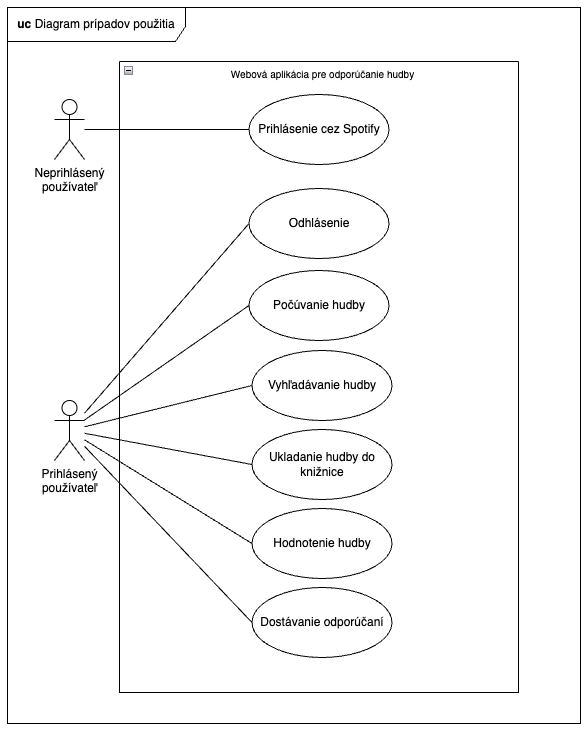
\includegraphics[scale=0.60]{img/usecase.png}
    \caption{Diagram prípadov použitia}
    \label{fig:usecase}
\end{figure}
V systéme rozlišujeme neprihláseného používateľa a prihláseného používateľa. Každý z týchto aktérov môže vykonávať určité akcie v aplikácii.

Neprihlásený používateľ má v aplikácii prístup iba k jednej funkcionalite. Jeho jedinou možnosťou je vykonať prihlásenie.
Prihlásenie do webovej aplikácie je realizované pomocou integrácie so službou Spotify. Ak používateľ nemá účet Spotify, nemôže sa prihlásiť. 

Po prihlásení do systému sa používateľovi sprístupnia všetky hlavné funkcie aplikácie. Prihlásený používateľ môže kedykoľvek systém opustiť prostredníctvom odhlásenia. Má možnosť prehrávať hudbu priamo v aplikácii, pričom prehrávanie je technicky zabezpečené prostredníctvom integrácie Spotify Web Playback SDK. Používateľ môže vyhľadávať hudobné skladby na a výsledky vyhľadávania sú získavané priamo z katalógu Spotify. Má taktiež prístup ku svojej knižnici z platformy Spotify. Dôležitou súčasťou je aj hodnotenie hudby, kde môže používateľ vyjadriť svoje preferencie a tieto hodnotenia sú následne využívané pri tvorbe personalizovaných odporúčaní. Na základe zozbieraných hodnotení, uloženej hudby a histórie počúvania systém automaticky generuje odporúčania na ďalšiu hudbu, ktorá by mohla používateľa zaujímať.

\subsection{Diagram tried}
\begin{figure}[!ht]
    \centering
    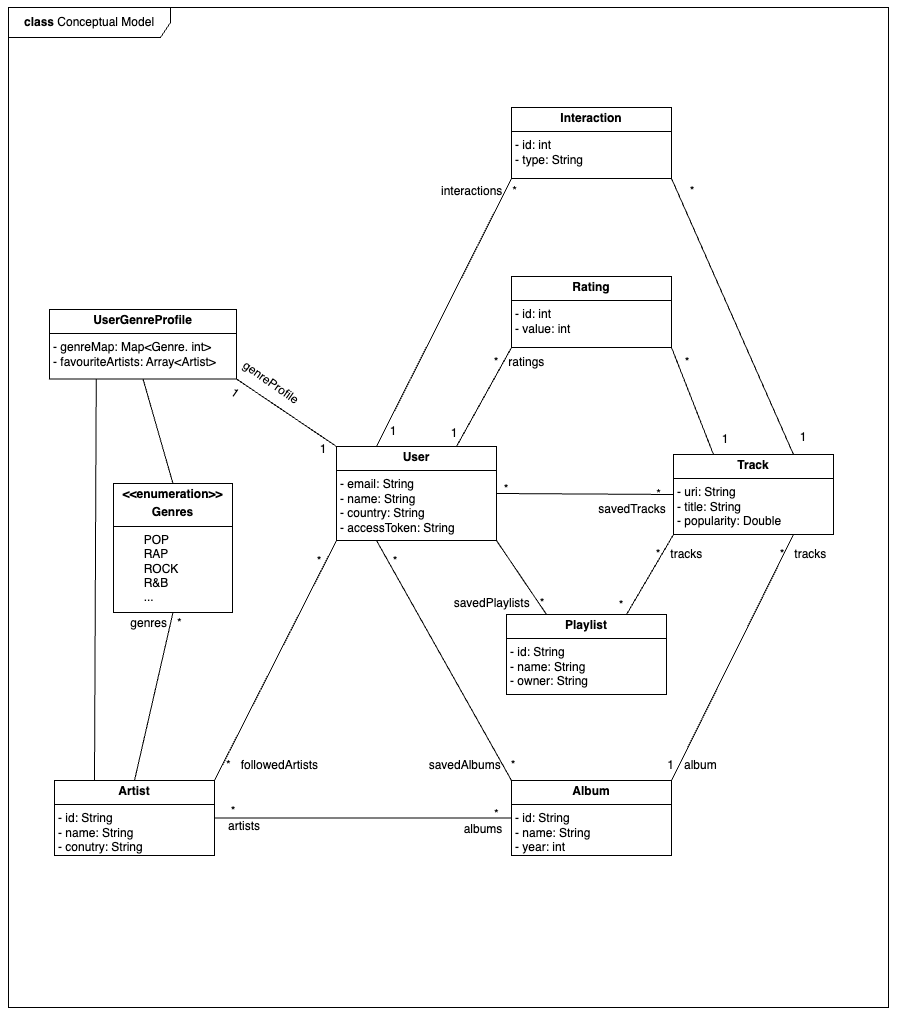
\includegraphics[scale=0.40]{img/class.png}
    \caption{Diagram tried}
    \label{fig:class}
\end{figure}
Na \ref{fig:class} 
Na OBR.(tuto odkomentovat obrazok) je znázornený diagram tried aplikácie použitý pri mojej implementácii. Hlavnou triedou tohto diagramu je trieda User, ktorá reprezentuje jednotlivých používateľov systému. Každý používateľ má vo svojom profile základné informácie, ako sú meno, email, krajina pôvodu a prístupový token pre Spotify Web API. Užívateľ v systéme je prepojedný s viacerými ďalšími entitami, pričom jeho hudobné preferencie a správanie sú kľúčové pre fungovanie odporúčacieho algoritmu.

Dôležitú úlohu pri personalizovaní odporúčaní zohráva trieda UserGenreProfile. Táto trieda obsahuje mapu žánrových preferencií konkrétneho používateľa, pričom ku každému žánru je priradená číselná hodnota reprezentujúca preferovaný rok v rámci obľúbeného žánru. V triede sa tiež nachádza zoznam obľúbených interpretov daného používateľa.

Samotná hudobná skladba je v systéme reprezentovaná ako Track. Uchováva informácie o jednotlivých skladbách vrátane ich názvu, URI a popularity. Skladby sú prepojené s ďalšími entitami, ako sú albumy a playlisty, a používateľ si ich môže ukladať medzi svoje obľúbené skladby alebo ich hodnotiť. Prepojenia medzi triedou User a Track zároveň umožňujú sledovať, aké skladby si používateľ uložil, aké skladby hodnotil, a aké interakcie s nimi mal (napríklad prehrávanie, preskakovanie či pridávanie do playlistov).

Okrem toho môže používateľ sledovať svojich obľúbených interpretov (trieda Artist), ukladať si albumy (trieda Album) či vytvárať a ukladať playlisty (trieda Playlist). Triedy Interaction a Rating obsahujú dáta o hodnoteniach a správaní používateľa.


\section{Implementačná časť}\label{sec:ImplementacnaCast}
V tejto časti bude popísaný celý proces implementácie od prvotného nastavenia, vzhľadu webovej aplikácie, až po  

\subsection{Použité nástroje a ich nastavenie}
Programovaniu aplikácie predchádzalo nastavenie a inštalácia potrebných nástrojov.

\subsubsection{PhpStorm}
PhpStorm bol využitý ako hlavné vývojové prostredie pre frontend aj backend. Pomáha s písaním kódu, kontrolou chýb a prácou so súbormi. PhpStorm som si vybral aj kvôli osobnej preferencii a predošlých skúsenostiach. Pre aktiváciu som použil školskú licenciu.

\subsubsection{npm}
npm je nástroj na správu balíčkov, ktorý sa používa na inštaláciu knižníc a spúšťanie vývojových skriptov. Je potrebný pre chod aplikácie a všetkých použitých knižníc. Nainštalovaný bol automaticky spolu s Node.js.

\subsubsection{Node.js}
Node.js slúži na spúšťanie JavaScript kódu na strane servera a je základom pre backend aj pre správu frontendu. Inštalácia bola vykonaná jednoducho cez príkazový riadok podľa oficiálnej dokumentácie.

\subsubsection{React a Vite}
Pre vývoj mojej webovej aplikácie som si zvolil React pre jeho komponentový prístup. Na inštaláciu a konfiguráciu projektu som využil nástroj Vite. Vite umožňuje jednoduché vytvorenie projektu pomocou šablón, vrátane šablóny pre React, ktorá automaticky nainštaluje potrebné závislosti. Vite taktiež umožňuje okamžitú aktualizáciu častí aplikácie počas vývoja bez potreby obnovenia celej stránky. 
Pre vytvorenie projektu som použil príkaz: \texttt{npm create vite@latest vite-app -- --template react}
Po vytvorení projektu som prešiel do jeho adresára a nainštaloval všetky závislosti pomocou \texttt{npm install}

\subsubsection{Github}
V projekte bol použitý git a platforma GitHub na správu verzovania zdrojového kódu, čo zabezpečilo zálohovanie a jednoduché obnovenie jednotlivých verzií aplikácie v prípade potreby. PhpStorm ponúka prehľadnú integráciu gitu, vďaka čomu bola správa zmien a synchronizácia so vzdialeným repozitárom prehľadná.

\subsubsection{Spotify Web API}
Spotify Web API je externá služba, ktorá poskytuje dáta o hudobných skladbách, interpretoch a umožňuje prehrávanie hudby v aplikácii. Na jeho používanie je potrebné zaregistrovať aplikáciu v Spotify Developer portáli a získať klientské údaje pre autentifikáciu.

\subsubsection{Knižnica spotify-web-api-node}
Táto knižnica slúži ako Node.js wrapper pre Spotify Web API, čo umožňuje jednoduchú komunikáciu so Spotify z backendu aj frontendu. Na jej používanie bol získaný prístupový token prostredníctvom autentifikačného toku Spotify s názvom Authorization Code Flow. Inštalovaná bola pomocou \texttt{npm install spotify-web-api-node} v zložkách client aj server.

\subsubsection{Knižnica react-spotify-web-plaback}
Táto knižnica poskytuje jednoduchý React komponent pre prehrávanie hudby pomocou Spotify Web Playback SDK. Umožňuje prehrávať skladby priamo v prehliadači a poskytuje ovládacie prvky ako play, pause, next a previous. Na jej fungovanie je potrebný prístupový token s príslušnými oprávneniami.
Inštalovaná bola v zložke client pomocou \texttt{npm install react-spotify-web-playback}.

\subsubsection{Knižnica Axios}
Knižnica Axios je populárny HTTP klient pre JavaScript, ktorý umožňuje jednoducho realizovať HTTP požiadavky z frontendu na backend alebo na externé API. Ponúka jednoduché rozhranie na posielanie GET, POST a ďalších typov požiadaviek. V tomto projekte sa Axios využíva najmä na komunikáciu medzi React frontendom a backendovým serverom, ako aj na získavanie údajov zo Spotify Web API. Knižnica bola nainštalovaná v zložke client pomocou príkazu \texttt{npm install axios}.

\subsubsection{Tailwind}
Tailwind CSS je jednoduchý nástroj na rýchle štýlovanie stránky priamo v HTML alebo JSX. Inštalovaný bol pomocou npm a umožňuje jednoducho meniť dizajn priamo v kóde bez písania zložitých CSS súborov.

\subsubsection{Docker pre databázu}
Na správu a spúšťanie MySQL databázy v rámci projektu bol použitý Docker, ktorý umožňuje jednoduché a izolované nasadenie databázového systému v kontajneri. Databáza je v projekte spustená ako samostatný kontajner podľa špecifikácie v konfiguračnom súbore (\texttt{docker-compose.yml}). Štruktúra databázy je definovaná v samostatnom súbore, ktorý obsahuje popis tabuliek a vzťahov medzi nimi. Použitie Dockeru výrazne uľahčuje spúšťanie a správu databázy počas vývoja aj nasadenia.


\subsection{Štruktúra projektu}
Projekt je rozdelený na dve hlavné časti – server (backend) a client (frontend). V priečinku server sa nachádzajú základné súbory backendu vrátane hlavného súboru server.js, ktorý poskytuje API pre autentifikáciu, odporúčania a interakciu s databázou aj Spotify. Súbor initialiseUserInDatabase.js slúži na naplnenie databázy pri prvom prihlásení používateľa. V priečinku recommender sú implementované jednotlivé odporúčacie algoritmy (explicit.js, implicit.js). Frontendová časť projektu je v priečinku client, kde sa v podpriečinku src nachádzajú React komponenty pre jednotlivé časti aplikácie, ako sú Albums.jsx, Artists.jsx, Dashboard.jsx, Recommendations.jsx a ďalšie, ktoré tvoria používateľské rozhranie. 

\subsection{Autorizácia a prihlásenie}
V mojej bakalárskej práci som implementoval autentifikáciu a autorizáciu používateľov prostredníctvom Spotify Web API s využitím Authorization Code Flow, čo je odporúčaný spôsob pre webové aplikácie, ktoré vyžadujú prístup k citlivým údajom používateľa a potrebujú obnovovať prístupové tokeny bez opätovného zásahu používateľa.

\begin{figure}[!ht]
    \centering
    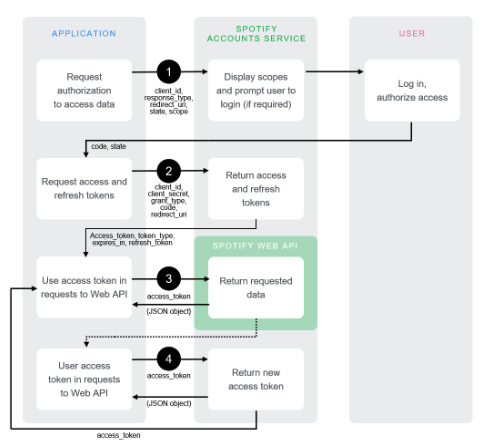
\includegraphics[scale=0.80]{img/auth.png}
    \caption{Authorization Code Flow pre Spotify Web API}
    \label{fig:auth}
    \cite{imgAuth}
\end{figure}

Authorization Code Flow je súčasťou protokolu OAuth 2.0 a prebieha v niekoľkých krokoch. Najprv aplikácia presmeruje používateľa na prihlasovaciu stránku Spotify, kde sa používateľ prihlási a udelí aplikácii požadované oprávnenia. Po úspešnom prihlásení a udelení oprávnení je používateľ presmerovaný späť na mnou preddefinovanú adresu s priloženým autorizačným kódom. Tento kód aplikácia následne použije na získanie prístupového tokenu a obnovovacieho tokenu prostredníctvom požiadavky na Spotify API. Prístupový token slúži na autentifikáciu ďalších požiadaviek voči Spotify API, zatiaľ čo obnovovací token umožňuje získanie nového prístupového tokenu po jeho exspirácii bez nutnosti opätovného prihlásenia používateľa.
V mojej implementácii je tento proces realizovaný na strane servera v súbore server.js. Po získaní autorizačného kódu od klienta server vytvorí inštanciu SpotifyWebApi s potrebnými konfiguračnými údajmi, vrátane clientId, clientSecret a redirectUri. Následne server zavolá metódu authorizationCodeGrant, ktorá vráti prístupový a obnovovací token. Tieto tokeny sú potom použité na získanie informácií o používateľovi prostredníctvom metódy getMe, čo umožňuje identifikáciu používateľa a jeho správu v databáze.

Dôležitou súčasťou procesu autorizácie sú tzv. scopes, ktoré definujú rozsah oprávnení, ktoré aplikácia požaduje od používateľa. V mojej aplikácii som využil napríklad tieto scopes:

    •	user-read-email – prístup k e-mailovej adrese používateľa,

    •	user-read-private – prístup k základným informáciám o profile používateľa,
	
    •	user-library-read a user-library-modify – čítanie a úprava knižnice používateľa,
	
    •	user-top-read – prístup k najčastejšie prehrávaným skladbám a interpretom,
	
    •	user-modify-playback-state – ovládanie prehrávania na zariadeniach používateľa.

Tieto scopes sú špecifikované pri presmerovaní používateľa na prihlasovaciu stránku Spotify a určujú, aké údaje a funkcie bude mať aplikácia k dispozícii po udelení oprávnení používateľom.

Implementácia Authorization Code Flow v mojej aplikácii zabezpečuje bezpečný a efektívny spôsob autentifikácie a autorizácie používateľov, čo je nevyhnutné pre poskytovanie personalizovaných odporúčaní a interakciu s používateľským účtom na Spotify.

\subsection{Štruktúra databázy}
Databázová štruktúra mojej aplikácie je realizovaná v MySQL a bola navrhnutá tak, aby vedela uchovávať všetky dôležité dáta potrebné pre tvorbu hudobných odporúčaní a evidovanie používateľského správania. Hlavnými tabuľkami databázy sú tabuľky artists (interpreti), genres (žánre), tracks (skladby) a users (používatelia), ktoré uchovávajú základné informácie o hudobnom obsahu a samotných používateľoch. Pre prepojenie údajov sú v databáze viaceré spojovacie tabuľky, ktoré prepájajú napríklad skladby s interpretmi, žánrami alebo používateľmi.

Z pohľadu používateľa sú kľúčové tabuľky interactions a ratings, ktoré slúžia na zaznamenávanie akcií ako hodnotenie skladieb, preskakovanie či ukladanie do knižnice. Evidujú sa tu aj informácie o najpočúvanejších skladbách a sledovaných interpretoch, uložených skladbách či playlistoch. Playlisty sú spravované samostatne, pričom každý playlist môže byť zameraný na konkrétny žáner a môže obsahovať viacero skladieb.

\subsection{Používateľské rozhranie}
Užívateľské rozhranie bolo navrhnuté pre jednoduchú interakciu s používateľa s aplikáciou. Rôzne časti aplikácie predstavím bližšie v tejto kapitole.

\subsubsection{Prihlásenie}
Stránka prihlásenie pozostáva z jednoduchého nadpisu a tlačidla na prihlásenie, ktoré presmeruje používateľa na prihlásenie cez platformu Spotify. Po úspšnom prihlásení je používateľ naspäť presmerovaný do aplikácie.

\subsubsection{Navigácia}
Po prihlásení je používateľovi sprístupnený navigačný panel na ľavej strane stránky ktorý má formu vertikálneho stĺpca. V hornej časti obsahuje používateľove meno s jeho profilovou fotkou a tlačidlo na odhlásenie. Toto často sa nachádza pole pre vyhľadávanie piesní a sekcia a tlačidla pre rôzne sekcie. Pod Toto častou sa nachádza pole pre vyhľadávanie piesní a sekcia S tlačidlami pre zobrazenie rôznych časti aplikácie ako napríklad obľúbené skladby playlisty a odporúčania.

\subsubsection{Hudobný prehrávač a hodnotenie}
V hornej časti stránky sa nachádza hudobný prehrávač ktorý umožňuje základné ovládanie prehrávania skladieb.
Pod ním sa nachádza sekcia umožňujúca hodnotenie ktorá má formu 5 hviezdičiek. Po kliknutí na daný počet hviezdičiek je uložená do databázy informácia o preferencií pre aktuálne hrajúcu skladbu.
Po kliknutí na daný počet hviezdičiek je uložená do databázy informácia o preferencií pre aktuálne hrajúcu skladbu.
\begin{figure}[!ht]
    \centering
    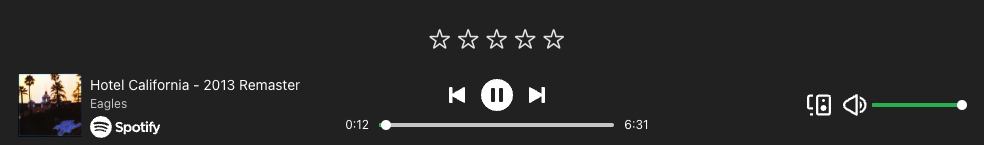
\includegraphics[scale=0.40]{img/prehravac.png}
    \caption{Hodnotenie a prehrávač}
    \label{fig:prehravac}
\end{figure}

\subsubsection{Vyhľadávanie}
Vyhľadávanie hudobného obsahu dostupného z platformy Spotify je umožnené pomocou vyhľadávacieho poľa v hornej časti navigačného panelu. Výsledky vyhľadávania sa zobrazujú v hlavnej časti stránky pod sekciou s hodnotením a sú aktualizované pri každej zmene vo vyhľadávanom reťazci.
\begin{figure}[!ht]
    \centering
    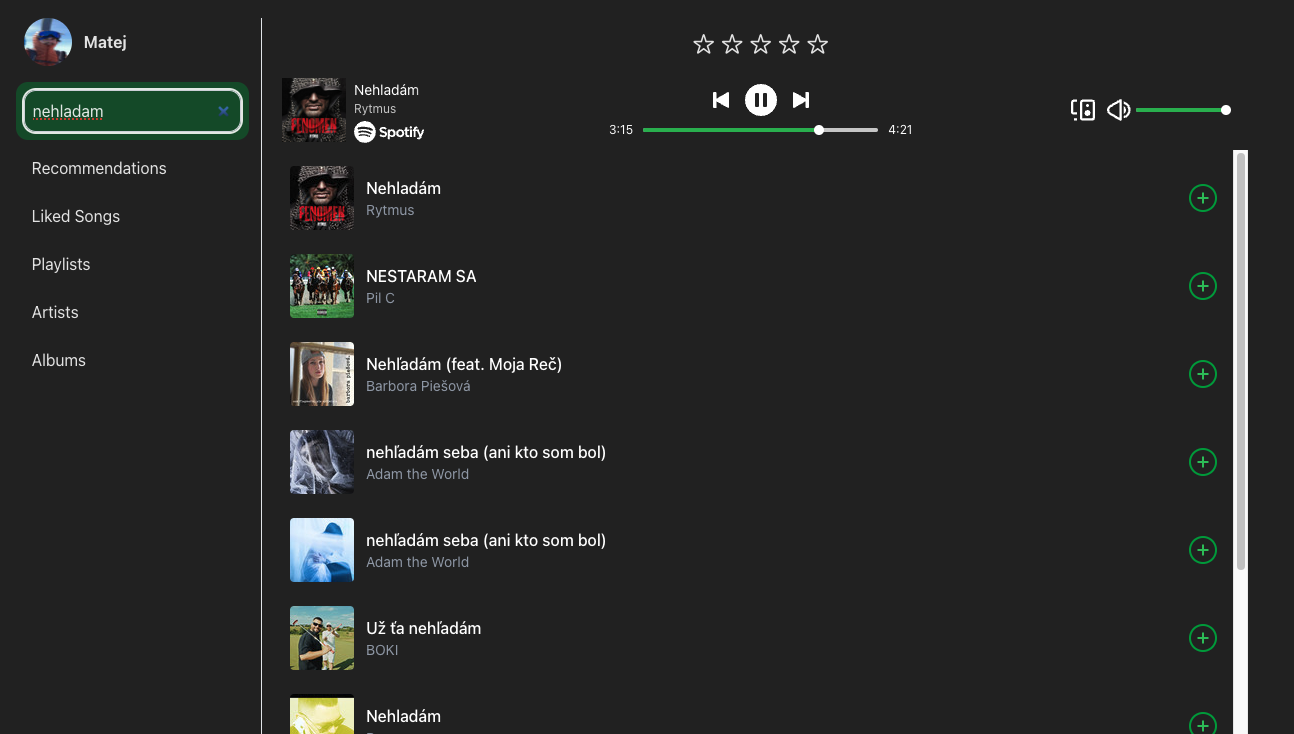
\includegraphics[scale=0.30]{img/hladam.png}
    \caption{Vyhľadávanie}
    \label{fig:hladam}
\end{figure}

\subsubsection{Odporúčané skladby}
Pod Sekciou vyhľadávania navigačnom paneli sa nachádza tlačidlo pre zobrazenie odporúčaných sklade. S tvojou stlačení sa v hlavnej časti stránky vygeneruje a zobrazí zoznam 20 skladieb, ktoré by sa používateľovi mohli páčiť. V každom riadku zobrazujúcom pieseň je aj tlačidlo pre pridanie do používateľovej knižnice, ktoré okrem pridania piesne do používateľovej knižnice na platforme spotify taktiež aj odosiela do databázy informáciu o používateľovej interakcii so skladbou.
\begin{figure}[!ht]
    \centering
    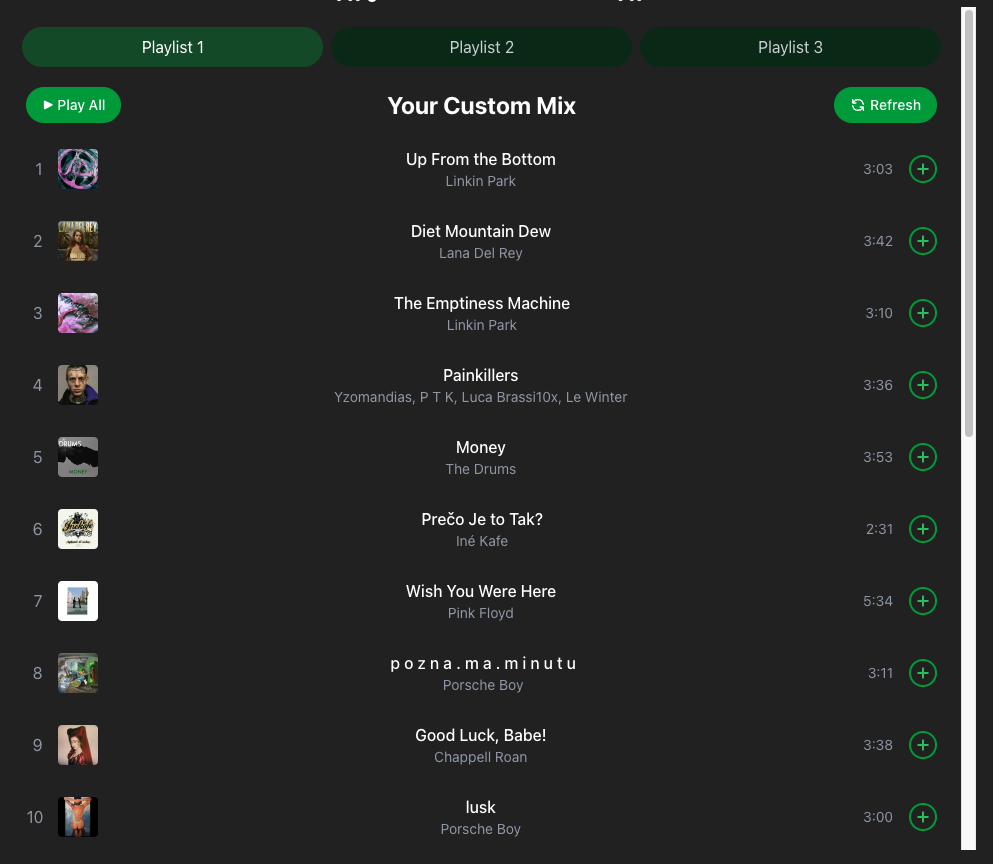
\includegraphics[scale=0.40]{img/odporucania.png}
    \caption{Odporúčané playlisty}
    \label{fig:odporucania}
\end{figure}

\subsubsection{Ostatné sekcie}
Stránka obsahuje ďalšie sekcie dostupné v navigačnom paneli, ktoré umožňujú používateľovi prehľadať svoju knižnicu na platforme Spotify. Používateľ mám prístup ku svojím obľúbeným skladbám, playlistom, interpretom a aj uloženým albumom.


\subsection{Odporúčací algoritmus}
V mojej bakalárskej práci som navrhol a implementoval systém odporúčania hudby, ktorý umožňuje porovnať tri prístupy vyhodnotenia používateľových preferencií: explicitné, implicitné a hybridné. Každý z týchto prístupov využíva odlišnú kombináciu údajov pre vytvorenie hudobného profilu používateľa.

Výstupom algoritmu je playlist, ktorý pozostáva z niekoľkých skupín skladieb, aby sa bola docielená rozmanitosť. Vytvorený playlist je zložený z troch hlavných typov skladieb:

	•	Aktuálne populárne skladby s najvyšším skóre podobnosti podľa žánrov a interpretov:
Tieto skladby sú najskôr vybrané z databázy. Sú to 4 playlisty s vyše 200 rôznymi skladbami, ktoré boli v čase implementácie populárne. Každá skladba je bodovaná na základe žánrovej podobnosti medzi používateľským profilom a skladbou a podľa popularity. Do playlistu sa vyberajú tie s najvyšším skóre, čím je zabezpečené, že odporúčané skladby by mali byť podobné vkusu používateľa, no zároveň má jemný vplyv na výpočet aj hodnota popularity z tabuľky. 

	•	Skladby vybrané zo žánrovo vhodných playlistov:
Pre každý zo zistených preferovaných žánrov používateľa sú vyhľadávané playlisty zodpovedajúce danému žánru a krajine. V databáze je vložených vyše 18 playlistov pre rôzne žánre. Dokopy je v týchto playlistoch vyše 2000 skladieb. Z každého takéhoto playlistu sú následne vyberané skladby podľa obdobia, v ktorom používateľ o daný žáner prejavoval najväčší záujem (štatisticky podľa výskytu hodnotených skladieb v rokoch — Q1, medián, Q3). Väčšina odporúčaných skladieb je preto z obdobia, ktoré by malo byť používateľovi blízke, pričom menšia časť je vybraná aj z okolitých rokov aby sa neznížila rozmanitosť. Používateľ tak môže objaviť nové skladby v rámci svojho obľúbeného žánru.
	
    •	Skladby od obľúbených interpretov:
Na základe najvyššie bodovaných interpretov v používateľskom profile algoritmus získava zo Spotify API najpopulárnejšie skladby každého z nich vzhľadom na lokáciu pouťívateľa. Z týchto skladieb sa do playlistu vyberá 5 náhodných, aby bol playlist doplnený aj o interpretov, o ktorých predpokladáme, že má používateľ najradšej a tým pádom by sa mu mali páčiť.


\subsubsection{Spracovanie explicitných hodnotení}
Explicitný odporúčací algoritmus využíva výhradne údaje, ktoré používateľ priamo poskytol alebo prejavil svojím správaním v aplikácii. Tieto údaje sú ukladané v databáze systému a pochádzajú zo štyroch základných zdrojov:
	•	Hodnotenia skladieb (ratings):
Používateľom udelené hodnotenia sú považované za najdôležitejší zdroj informácií o preferenciách, pretože priamo vyjadrujú, do akej miery sa mu skladba páčila. Pri výpočte profilu majú jednotlivé hodnotenia rôznu váhu:
	•	Hodnotenie 5 prispieva 5 bodmi,
	•	hodnotenie 4 prispieva 3 bodmi,
	•	hodnotenie 3 prispieva 1 bodom.
Ostatné hodnotenia sa pri výpočte preferenčného profilu vynechávajú. Body sa prirátajú ku každému žánru a interpretovi, ktorý je priradený k danej skladbe.
	•	Uložené skladby (saved tracks):
V databáze sa, pre ušetrenie miesta, nachádza 50 posledných skladieb, ktoré používateľ uložil do svojej knižnice. Každá skladba prispieva žánru a interpretovi 3 bodmi.
	•	Playlisty používateľa:
Skladby nachádzajúce sa v playlistoch vytvorených alebo uložených používateľom prispievajú ku skóre žánru a interpreta jedným bodom. Táto váha je najnižšia, keďže playlistu nemusí byť uložený kvôli tomu, že obsahuje iba také skladby, ktoré sa používateľovi páčia.
	•	Sledovaní interpreti (followed artists):
Každý sledovaný interpret prispieva k jeho skóre 5 bodov, pretože sledovanie interpreta je považované za silný prejav záujmu.

Výsledné skóre sa sčítava pre každý žáner a interpreta naprieč všetkými zdrojmi, pričom výsledkom je preferenčný profil používateľa v podobe objektu userProfile. Tento objekt obsahuje:
	•	Zoznam najvýraznejších interpretov (maximálne 5) podľa bodového skóre.
        •	Zoznam najvýraznejších žánrov (maximálne 10) podľa celkového skóre.
        
Pre každý žáner je zistený medián a hodnoty Q1 a Q3, ktoré by mali obsahovať preferenciu rokov vydaných skladieb v rámci žánru, ktoré sa používateľovi páčia.

\subsubsection{Spracovanie implicitných hodnotení}

Implicitný odporúčací algoritmus vyhodnocuje preferencie používateľa na základe jeho správania počas používania aplikácie a dlhodobo najviac počúvaných skladieb. Údaje o správaní sú uložené v databáze systému a pochádzajú z rôznych druhov interakcií používateľa so skladbami za posledných 30 dní. Konkrétne ide o tieto typy akcií:
	•	Pridanie skladby do knižnice: Táto akcia je vnímaná ako silný prejav záujmu o skladbu, a preto prispieva žánru a interpretovi 3 bodmi.
	•	Prehratie skladby: Každé prehratie skladby prispieva k skóre žánru a interpreta 1 bodom, čo odráža bežnú mieru záujmu.
	•	Preskočenie skladby: Ak používateľ skladbu preskočí, žánru aj interpretovi sa odráta 2 body, keďže ide o signál nezáujmu.
	•	Odstránenie skladby z knižnice: Táto akcia má najväčšiu negatívnu váhu a priraďuje žánru aj interpretovi -3 body.

Hodnoty všetkých interakcií za posledných 30 dní sa sčítavajú pre každý žáner a interpreta. K tomuto skóre sa následne pripočítavajú aj body za najpočúvanejšie skladby v dlhodobom horizonte (v databáze sa nachádza 100 najpočúvanejších skladieb daného používateľa), ktoré reprezentujú dlhodobý vkus používateľa – každému žánru a interpretovi je za výskyt v tabuľke top tracks pripočítaný 1 bod. Body získané z krátkodobých a dlhodobých interakcií sa sčítavajú, pričom najviac sa zohľadňujú aktuálne správanie a preferencie.

Výsledkom je preferenčný profil používateľa v podobe objektu userProfile, ktorý obsahuje:
	•	Zoznam najvýraznejších interpretov (maximálne 5) podľa bodového skóre,
	•	Zoznam najvýraznejších žánrov (maximálne 10) podľa celkového skóre.

Pre každý žáner sa, podobne ako pri explicitných hodnoteniach, zisťuje medián a kvartily (Q1, Q3) rokov vydania skladieb, ktoré patria do príslušného žánru a boli počúvané alebo inak preferované. 


\subsubsection{Hybridný prístup spracovania hodnotení}
Profil používateľa pri hybridnom vyhodnotení vzniká kombinovaním profilov, ktoré boli samostatne vytvorené explicitným aj implicitným odporúčacím algoritmom. Pomocou funkcie mergeProfiles sa tieto dva profily spoja do jedného výsledného profilu. Táto funkcia najprv zoberie zoznam žánrov z explicitného aj implicitného profilu a vypočíta vážený priemer štatistík (ako sú Q1, medián a Q3 rok výskytu skladieb v danom žánri). Pri výpočte sa  explicitným dátam priraďuje vyššia váha (0.7) a implicitným nižšia (0.3).

Pre interpretov sa profily jednoducho spoja du zoznamu všetkých interpretov z oboch profilov. Výsledkom je nový objekt userProfile, ktorý kombinuje silné stránky oboch prístupov.


\section{Testovanie a výsledky}\label{sec:TestovanieVysledky}
V tejto časti vysvetlím spôsob testovania rôznych prístupov hodnotenia používateľských preferencií v mojej aplikácii a vyvodím závery z výsledkov testovania.

\subsection{Výber typu testovania}
Pri návrhu testovania som si vyberal z viacerých prístupov, akými sa dajú hodnotiť odporúčacie systémy. Každý z nich má svoje výhody a nevýhody:
	
    •	Automatizované testovanie – Tento prístup používa simulované dáta alebo predpripravené scenáre, kde systém „testuje sám seba“ podľa presne určených pravidiel. Výhodou je rýchlosť a jednoduchá opakovateľnosť. Nevýhodou však je, že takéto testovanie nevie zachytiť skutočné pocity a preferencie naozajstných používateľov. Pri testovaní položiek, ktoré človek vníma subjektívne (ako napríklad v mojom prípade hudba) by takýto typ testovania bol tažko interpretovateľný.

    •	A/B testovanie – Tento spôsob je bežný napríklad v online službách, kde sa veľká skupina používateľov rozdelí na viacero častí a každá z nich dostane inú verziu odporúčaní. Je to vhodné pre veľké aplikácie s tisíckami používateľov. V mojom prípade, kde testujem webovú aplikáciu na malej vzorke ľudí, by tento prístup nebol dostatočnú výpovednú hodnotu.

    •	Používateľské štúdie a asistované testovanie – Tento prístup je vhodný práve pri menšom počte testerov a keď potrebujem získať podrobnú spätnú väzbu. Tester používa aplikáciu, hodnotí odporúčania a môže detailne popísať svoje pocity, čo je pre účely tejto práce ideálne.

Preto som sa rozhodol pre asistované testovanie – každý tester bude používať moju aplikáciu, do ktorej sa prihlási so svojím Spotify premium účtom. Spotify v mojom projekte umožňuje prístup pre maximálne 25 rôznych účtov. Tester bude najskôr simulovať bežné správanie, kvôli potrebe naplnenia databázy dátami a až následne si nechá vygenerovať playlisty s odporúčanými skladbami. Po vypočutí odporúčaných skladieb vyhodnotí kvalitu odporúčaní pomocou dotazníka. Typ takéhoto testovania je celkom časovo náročný, ale výsledky sú lepšie interpretovateľné a budú postavené na spätnej väzbe reálnych používateľov.

\subsection{Testovací scenár}
Testovanie prebiehalo podľa vopred stanoveného scenára pre zachovanie čo najväčšej podobnosti podmienok počas testovanie, avšak nebolo možné docieliť zakaždým rovnaký priebeh kvôli rozdielom v spôsobe počúvania hudby medzi jednotlivými používateľmi. Vygenerované zoznamy skladieb boli vždy zobrazené v rovnakom poradí, o čom však používateľ nevedel. Prvý zoznam je bol vygenerovaný na základe implicitných hodnotení, druhý na základe hybridných a tretí na základe explicitných. 

\subsubsection{Postup testovania}

    1.  Používateľ sa prihlási pomocou svojho Spotify Premium účtu do testovanej webovej aplikácie, pri tomto kroku sa databáza napĺňa niektorými používateľskými dátami zo Spotify účtu používateľa.

    2.	Po úspešnom prihlásení je používateľ požiadaný, aby po dobu 10 minút simuloval bežné používanie hudobnej aplikácie, to znamená púšťanie, preskakovanie skladieb, ukladanie obľúbených piesní, hodnotenie skladieb a podobne.

    3. Následne je požiadaný aby ohodnotil minimálne 10 skladieb podľa vlastného výberu, ak už tak neurobil.

    4.	Po tejto fáze, je požiadaný, aby si kliknutím na tlačidlo "Get Recommendations" nechal vygenrovať odporúčania. Odporúčací systém následne vygeneruje tri playlisty, každý po 20 skladieb. Každý z týchto playlistov je vytvorený iným prístupom vyhodnotenia jeho preferencií, pričom používateľ nevie, ktorým spôsob boli dané playlisty vytvorené.

    5.	Tester si postupne prehrá skladby vo všetkých troch zoznamoch skladieb. Po vypočutí každého z nich vyplní časť dotazníka zameranú na spokojnosť s konkrétnym zoznamom skladieb.

    6.	Po vypočutí a ohodnotení všetkých playlistov používateľ odošle dotazník na ďalšie spracovanie a môže sa odhlásiť z webovej aplikácie.

\subsection{Dotazník}
Testujúci používatelia boli požiadaní o vyplnenie dotazníku. Dotazník slúži na zistenie spätnej väzby o kvalite odporúčaní každého testovaného algoritmu. Vždy po vypočutí skladieb z jednotlivého vygenerovaného playlistu, používatelia odpovedali na tri otázky. Na prvé dve otázky odpovedali označením čísla na škále od 1 do 7, v tretej otázke boli požiadaní o uvedenie presného počtu skladieb. Tieto otázky zneli nasledovne:
    
    •	Ako by si celkovo ohodnotil odporúčania v tomto zozname?

    •	Ako veľmi ti odporúčania pripomínali tvoj bežný hudobný vkus?
	
    •	Koľko skladieb z odporúčaného zoznamu by si pridal do svojej knižnice?

\begin{figure}[!ht]
    \centering
    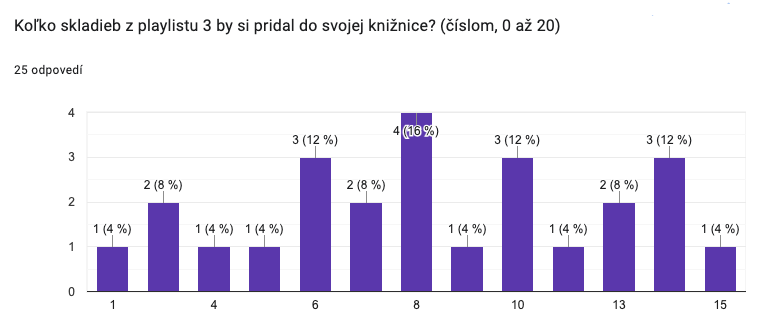
\includegraphics[scale=0.40]{img/uloz3.png}
    \caption{Odpovede na otázku č.5, playlist 3}
    \label{fig:uloz3}
\end{figure}



\subsection{Voľba metodiky evaluácie}
Pre vyhodnotenie výsledkov spokojnosti s jednotlivými algoritmami bolo potrebné najskôr rozhodnúť, aké štatistické metódy sú najvhodnejšie pre tento účel. Pre jednoduché porovnanie je možné použiť obyčajný priemer hodnôt pre každú otázku na určenie odporúčania s najvyššími priemernými známkami od používateľov. Pre väčší kontext bolo však potrebné zistiť, či medzi výslednými hodnotami bol aj štatisticky významný rozdiel. 

Prvým krokom bolo zistiť, či dáta majú normálne rozdelenie, čo je dôležité pre výber ďalšieho postupu. Pre tento účel som použil Shapiro-Wilkov test. Ak výsledky testu normality ukázali, že dáta sú normálne rozdelené, mohol sa použiť ANOVA test, ktorý vie porovnať odpovede jednej otázky pre všetky typy odporúčaní naraz a zistiť, či sú medzi nimi štatisticky významné rozdiely. Ak normalita nebola splnená, použil som Friedmanov test, ktorý je na tento účel vhodný, ak dáta nemajú normálne rozdelenie.

Ak niektorý z týchto testov ukázal, že existuje štatisticky významný rozdiel medzi porovnávanými algoritmami, pokračovalo sa párovým porovnávaním jednotlivých algoritmov navzájom. Pri ANOVA teste som na to využil Turkeyho test, a pri Friedmanovom teste som použil párové Wilcoxonove testy. Týmito testami bolo možné presne určiť, medzi ktorými dvojicami algoritmov sa v hodnotení vyskytli štatisticky významné rozdiely.


\subsection{Evaluácia}
Závery som vyvodzoval na základe analýzy troch typov otázok z dotazníka pre každý algoritmus. Prvou skúmanou otázkou bola celková spokojnosť s playlistom. Druhá otázka hodnotila podobnosť playlistu s hudobným vkusom používateľa a tretia sledovala počet skladieb pridaných do knižnice.

\subsubsection{Spokojnosť s vygenerovanými odporúčaniami}

Na úvod bola pomocou Shapiro-Wilk testu overená normalita rozdielov medzi hodnoteniami spokojnosti s odporúčaniami troch algoritmov (Tabuľka~\ref{tab:shw1}). Všetky porovnávané dvojice mali p-hodnotu väčšiu ako 0,05, takže možno predpokladať, že rozdiely medzi hodnoteniami sú normálne rozdelené. Na základe toho bolo možné použiť parametrický test – ANOVA pre opakované merania.

\begin{table}[h!]
  \caption{Shapiro-Wilk test normality – celková spokojnosť}
  \label{tab:shw1}
  \centering
  \begin{tabular}{@{}lrrc@{}}
    \toprule
    \textbf{Porovnávané dvojice} & \textbf{Shapiro-Wilk štatistika} & \textbf{p-hodnota} & \textbf{p > 0,05} \\
    \midrule
    Implicit -- Hybrid & 0{,}950 & 0{,}25 & Áno \\
    Implicit -- Explicit & 0{,}930 & 0{,}082 & Áno \\
    Hybrid -- Explicit & 0{,}946 & 0{,}202 & Áno \\
    \bottomrule
  \end{tabular}
\end{table}

Výsledok ANOVA testu (Tabuľka~\ref{tab:anova_hod}) ukázal, že existuje štatisticky významný rozdiel v spokojnosti medzi jednotlivými algoritmami (F = 12{,}41, p < 0{,}001).

\begin{table}[h!]
  \caption{ANOVA – celková spokojnosť}
  \label{tab:anova_hod}
  \centering
  \begin{tabular}{@{}lrrc@{}}
    \toprule
    \textbf{Test} & \textbf{F-hodnota / t-štatistika} & \textbf{p-hodnota} & \textbf{p < 0{,}05} \\
    \midrule
    ANOVA & 12{,}41 & 0{,}000 & Áno \\
    \bottomrule
  \end{tabular}
\end{table}

Post-hoc analýza (Tabuľka~\ref{tab:posthoc_hod}) s Bonferroniho korekciou ukázala, že spokojnosť s odporúčaniami bola štatisticky významne rozdielna medzi algoritmom Implicit a Hybrid (p = 0{,}001), ako aj medzi algoritmom Implicit a Explicit (p = 0{,}003). Naopak, medzi algoritmami Hybrid a Explicit rozdiel zistený nebol (p = 1{,}000).

\begin{table}[h!]
  \caption{Post-hoc testy (párové porovnania) – celková spokojnosť}
  \label{tab:posthoc_hod}
  \centering
  \begin{tabular}{@{}lrrc@{}}
    \toprule
    \textbf{Porovnávané dvojice} & \textbf{t-štatistika} & \textbf{p-hodnota (Bonferroni)} & \textbf{p < 0{,}05} \\
    \midrule
    Implicit -- Hybrid & -4{,}38 & 0{,}001 & Áno \\
    Implicit -- Explicit & -3{,}78 & 0{,}003 & Áno \\
    Hybrid -- Explicit & 0{,}94 & 1{,}000 & Nie \\
    \bottomrule
  \end{tabular}
\end{table}

Používatelia hodnotili algoritmus Implicit z hľadiska spokojnosti s odporúčaniami štatisticky odlišne ako zvyšné dva algoritmy. Hybrid a Explicit boli z pohľadu spokojnosti hodnotené podobne.


\subsubsection{Podobnosti s hudobným vkusom používateľa}
Na začiatku bola overená normalita rozdielov medzi hodnoteniami vkusu pre jednotlivé algoritmy (Tabuľka~\ref{tab:shw_vkus}). Výsledky ukázali, že rozdiely neboli normálne rozdelené vo väčšine prípadov (iba rozdiel Implicit – Explicit bol tesne normálny). Preto bol na porovnanie spokojnosti s odporúčaniami použitý neparametrický Friedmanov test.

\begin{table}[h!]
  \caption{Shapiro-Wilk test normality – podobnosť vkusu}
  \label{tab:shw2}
  \centering
  \begin{tabular}{@{}lrrc@{}}
    \toprule
    \textbf{Porovnávané dvojice} & \textbf{Shapiro-Wilk štatistika} & \textbf{p-hodnota} & \textbf{p > 0{,}05} \\
    \midrule
    Implicit -- Hybrid & 0{,}910 & 0{,}031 & Nie \\
    Implicit -- Explicit & 0{,}924 & 0{,}063 & Áno \\
    Hybrid -- Explicit & 0{,}818 & 0{,}000 & Nie \\
    \bottomrule
  \end{tabular}
\end{table}

Friedmanov test (Tabuľka~\ref{tab:friedman_vkus}) ukázal, že medzi hodnoteniami vkusu existuje štatisticky významný rozdiel pretože, p = 0{,}002.

\begin{table}[h!]
  \caption{Friedmanov test – vkus}
  \label{tab:friedman_vkus}
  \centering
  \begin{tabular}{@{}lrrc@{}}
    \toprule
    \textbf{Test} & \textbf{Testovacia štatistika} & \textbf{p-hodnota} & \textbf{p < 0{,}05} \\
    \midrule
    Friedman & 12{,}45 & 0{,}002 & Áno \\
    \bottomrule
  \end{tabular}
\end{table}

Post-hoc analýza s použitím Wilcoxonových párových testov (Tabuľka~\ref{tab:posthoc_vkus}) ukázala, že spokojnosť s odporúčaniami bola štatisticky významne odlišná medzi algoritmami Implicit a Hybrid (p = 0{,}004) a tiež medzi Implicit a Explicit (p = 0{,}008).
Medzi algoritmami Hybrid a Explicit nebol zistený významný rozdiel (p = 1{,}000).

\begin{table}[h!]
  \caption{Post-hoc testy (Wilcoxon, Bonferroni) – vkus}
  \label{tab:posthoc_vkus}
  \centering
  \begin{tabular}{@{}lrrc@{}}
    \toprule
    \textbf{Porovnávané dvojice} & \textbf{Wilcoxon štatistika} & \textbf{p-hodnota (Bonferroni)} & \textbf{p < 0{,}05} \\
    \midrule
    Implicit -- Hybrid & 32{,}50 & 0{,}004 & Áno \\
    Implicit -- Explicit & 30{,}50 & 0{,}008 & Áno \\
    Hybrid -- Explicit & 53{,}50 & 1{,}000 & Nie \\
    \bottomrule
  \end{tabular}
\end{table}

Používatelia hodnotili algoritmus Implicit z hľadiska podobnosti hudobného vkusu štatisticky inak ako zvyšné dva algoritmy. Hybrid a Explicit boli hodnotené podobne.


\subsubsection{Počet skladieb pridaných do knižnice}
Na začiatku bola overená normalita rozdielov medzi hodnoteniami uložených skladieb (Tabuľka~\ref{tab:shw_uloz}). Výsledky ukázali, že rozdiel Hybrid – Explicit nie je normálne rozdelený, preto bol na porovnanie použitý neparametrický Friedmanov test.

\begin{table}[h!]
  \caption{Shapiro-Wilk test normality – uložené skladby}
  \label{tab:shw_uloz}
  \centering
  \begin{tabular}{@{}lrrc@{}}
    \toprule
    \textbf{Porovnávané dvojice} & \textbf{Shapiro-Wilk štatistika} & \textbf{p-hodnota} & \textbf{p > 0{,}05} \\
    \midrule
    Implicit -- Hybrid & 0{,}967 & 0{,}570 & Áno \\
    Implicit -- Explicit & 0{,}978 & 0{,}842 & Áno \\
    Hybrid -- Explicit & 0{,}879 & 0{,}007 & Nie \\
    \bottomrule
  \end{tabular}
\end{table}

Friedmanov test (Tabuľka~\ref{tab:friedman_uloz}) ukázal, že medzi algoritmami existuje štatisticky významný rozdiel v počte uložených skladieb, pretože p = 0{,}002.

\begin{table}[h!]
  \caption{Friedmanov test – uložené skladby}
  \label{tab:friedman_uloz}
  \centering
  \begin{tabular}{@{}lrrc@{}}
    \toprule
    \textbf{Test} & \textbf{Testovacia štatistika} & \textbf{p-hodnota} & \textbf{p < 0{,}05} \\
    \midrule
    Friedman & 12{,}65 & 0{,}002 & Áno \\
    \bottomrule
  \end{tabular}
\end{table}

Post-hoc analýza (Tabuľka~\ref{tab:posthoc_uloz}) s použitím Wilcoxonových párových testov a Bonferroniho korekcie ukázala, že štatisticky významný rozdiel bol iba medzi algoritmami Implicit a Hybrid (p = 0{,}004).
Medzi dvojicami Implicit – Explicit a Hybrid – Explicit rozdiel významný nebol.
    
\begin{table}[h!]
  \caption{Post-hoc testy (Wilcoxon, Bonferroni) – uložené skladby}
  \label{tab:posthoc_uloz}
  \centering
  \begin{tabular}{@{}lrrc@{}}
    \toprule
    \textbf{Porovnávané dvojice} & \textbf{Wilcoxon štatistika} & \textbf{p-hodnota (Bonferroni)} & \textbf{p < 0{,}05} \\
    \midrule
    Implicit -- Hybrid & 33{,}50 & 0{,}004 & Áno \\
    Implicit -- Explicit & 75{,}00 & 0{,}164 & Nie \\
    Hybrid -- Explicit & 66{,}00 & 0{,}082 & Nie \\
    \bottomrule
  \end{tabular}
\end{table}

Používatelia si ukladali skladby významne inak v prípade algoritmov Implicit a Hybrid, ostatné rozdiely štatisticky významné neboli.


\subsubsection{Zhrnutie výsledkov}
Na základe výsledkov analýzy a meraní, najlepšie výsledky vo všetkých troch sledovaných oblastiach (celková spokojnosť, podobnosť s hudobným vkusom a počet skladieb pridaných do knižnice) dosiahol hybridný algoritmus. Hybridný algoritmus získal najvyššie priemerné hodnotenia pri celkovej spokojnosti (5,84), podobnosti s hudobným vkusom (5,40) aj v počte skladieb pridaných do knižnice (9,80). Výsledky štatistických testov preukázali významný rozdiel medzi hybridným algoritmom najmä v porovnaní s implicitným algoritmom. Explicitný algoritmus mal síce v prvých dvoch otázkach podobné výsledky ale, tým, že existovala významná odchýlka medzi ním a hybridným algoritmom v otázke počtu pridaných skladieb, môžem konštatovať, že hybridné hodnotenie používateľských preferencií je najvhodnejšie pre hudobné aplikácie.

\subsubsection{Odporúčanie pre využitie}
Ak je cieľom zvýšiť spokojnosť používateľov, zabezpečiť čo najvyššiu relevanciu odporúčaní a zvýšiť počet skladieb, ktoré si používatelia pridajú do knižnice, je vhodné použiť odporúčací systém, ktorý používa implicitné aj explicitné hodnotenia pre výpočet vhodnosti odporúčaní. Takýto systém je podľa výsledkov tejto evaluácie presnejší než čisto implicitné alebo explicitné riešenia. V praxi to znamená, že hudobné aplikácie by mali umožniť používateľom hodnotiť skladby ale zároveň aj zohľadňovať ich správanie (počúvanie, preskakovanie, vyhľadávanie). Využie oboch typov informácií vedie k lepším a relevantnejším odporúčaniam.


